% THIS IS SIGPROC-SP.TEX - VERSION 3.1
% WORKS WITH V3.2SP OF ACM_PROC_ARTICLE-SP.CLS
% APRIL 2009
%
% It is an example file showing how to use the 'acm_proc_article-sp.cls' V3.2SP
% LaTeX2e document class file for Conference Proceedings submissions.
% ----------------------------------------------------------------------------------------------------------------
% This .tex file (and associated .cls V3.2SP) *DOES NOT* produce:
%       1) The Permission Statement
%       2) The Conference (location) Info information
%       3) The Copyright Line with ACM data
%       4) Page numbering
% ---------------------------------------------------------------------------------------------------------------
% It is an example which *does* use the .bib file (from which the .bbl file
% is produced).
% REMEMBER HOWEVER: After having produced the .bbl file,
% and prior to final submission,
% you need to 'insert'  your .bbl file into your source .tex file so as to provide
% ONE 'self-contained' source file.
%
% Questions regarding SIGS should be sent to
% Adrienne Griscti ---> griscti@acm.org
%
% Questions/suggestions regarding the guidelines, .tex and .cls files, etc. to
% Gerald Murray ---> murray@hq.acm.org
%
% For tracking purposes - this is V3.1SP - APRIL 2009

%%\documentclass{sig-alternate}
%%hp cr: using www2012-accepted
\documentclass{www2012-accepted}
\usepackage{cite}
\usepackage{url}
\usepackage{hyperref}
%\usepackage[table]{xcolor} 
\usepackage{times}
\usepackage{color}
%\usepackage{multirow} %mk
\usepackage{verbatim}

\usepackage{multirow}
\begin{document}
\clubpenalty=10000 
\widowpenalty = 10000
\newcommand{\xhdr}[1]{{\vspace{6pt}\noindent\textbf{\textit{#1}}}}

\newcommand{\soic}{\affaddr{School of Informatics \& Computing}\\ 
\affaddr{Indiana University}\\
\affaddr{Bloomington, IN}\\}

\title{Mining Photo-sharing Websites to Study\\ Ecological Phenomena}


\numberofauthors{4} %  in this sample file, there are a *total*
% of EIGHT authors. SIX appear on the 'first-page' (for formatting
% reasons) and the remaining two appear in the \additionalauthors section.
%

\author{
% You can go ahead and credit any number of authors here,
% e.g. one 'row of three' or two rows (consisting of one row of three
% and a second row of one, two or three).
%
% The command \alignauthor (no curly braces needed) should
% precede each author name, affiliation/snail-mail address and
% e-mail address. Additionally, tag each line of
% affiliation/address with \affaddr, and tag the
% e-mail address with \email.
%
% 1st. author
\alignauthor
%Anonymous CIKM submission \\
 Haipeng Zhang\\
 \soic
 \email{zhanhaip@indiana.edu}
 % 2nd. author
 \alignauthor
 Mohammed Korayem\\
 \soic
 \email{mkorayem@indiana.edu}
 % 3rd. author
 \alignauthor 
 David J. Crandall \\
 \soic
 \email{djcran@indiana.edu}
 \and
 \alignauthor
 Gretchen LeBuhn \\
 \affaddr{Department of Biology} \\
 \affaddr{University of California} \\
 \affaddr{San Francisco, CA} 
 \email{lebuhn@sfsu.edu}
}

% There's nothing stopping you putting the seventh, eighth, etc.
% author on the opening page (as the 'third row') but we ask,
% for aesthetic reasons that you place these 'additional authors'
% in the \additional authors block, viz.
%\additionalauthors{Additional authors: John Smith (The Th{\o}rv{\"a}ld Group,
%email: {\texttt{jsmith@affiliation.org}}) and Julius P.~Kumquat
%(The Kumquat Consortium, email: {\texttt{jpkumquat@consortium.net}}).}
%\date{30 July 1999}
% Just remember to make sure that the TOTAL number of authors
% is the number that will appear on the first page PLUS the
% number that will appear in the \additionalauthors section.

\maketitle
\begin{abstract}
The popularity of social media websites like Flickr
and Twitter has created enormous collections of user-generated content
online. Latent in these content collections are observations of the
world: each photo is a visual snapshot of what the world looked like
at a particular point in time and space, for example, while each tweet
is a textual expression of the state of a person and his or her
environment. Aggregating these observations across millions
of social sharing users could lead to new techniques for large-scale
monitoring of the state of the world and how it is changing over
time. In this paper we step towards that goal, showing that by
analyzing the tags and image features of geo-tagged, time-stamped
photos we can measure and quantify the occurrence of ecological
phenomena including ground snow cover, snow fall and vegetation
density.  We compare several techniques for dealing with the large
degree of noise in the dataset, and show how machine learning can be
used to reduce errors caused by misleading tags and ambiguous visual
content. We evaluate the accuracy of these techniques by comparing to
ground truth data collected both by surface stations and by
Earth-observing satellites. Besides the immediate application to
ecology, our study gives insight into how to accurately crowd-source
other types of information from large, noisy social sharing datasets.
\end{abstract}

% A category with the (minimum) three required fields
\category{H.2.8}{Database Management}{Database Applications}[Data
Mining, Image Databases, Spatial Databases and GIS]
\category{I.4.8}{Image Processing and Computer Vision}{Scene Analysis}

\terms{Measurement, Theory}

\keywords{Data mining, social media, photo collections, crowd-sourcing, ecology} % NOT required for Proceedings

\newcommand{\leaveout}[1]{}

\newenvironment{packed_itemize}{
\begin{itemize}
  \setlength{\itemsep}{0pt}
  \setlength{\parskip}{0pt}
  \setlength{\parsep}{0pt}
\vspace{-4pt}
}{\end{itemize}}

\vspace{12pt}
\section{Introduction}

The popularity of social networking websites has grown dramatically
over the last few years, creating enormous collections of
user-generated content online. Photo-sharing sites have become
particularly popular: Flickr and Facebook alone have amassed an
estimated 100 billion images, with over 100 million new images
uploaded every day~\cite{Kremerskothen11}.  People use these
sites to share photos with family and friends, but in the process they
are creating immense public archives of information about the world:
each photo is a record of what the world looked like at a particular
point in time and space.  When combined together, the billions of
photos on these sites combined with metadata including timestamps,
geo-tags, and captions are a rich untapped source of information about
the state of the world and how it is changing over
time.

Recent work has studied how to mine passively-collected data
from social networking and microblogging websites to make estimates
and predictions about world events, including tracking the spread of
disease~\cite{ginsberg09flu}, monitoring for fires and
emergencies~\cite{delongueville09}, predicting product adoption rates
and election outcomes~\cite{jin10prediction}, and estimating aggregate
public mood~\cite{oconnor10mood,bollen11twitter}. In most of these
studies, however, there is either little ground truth available to
judge the quality of the estimates and predictions, or the available
ground truth is an indirect proxy (e.g. since no aggregate public mood
data exists, \cite{oconnor10mood} evaluates against opinion polls,
while~\cite{bollen11twitter} compares to stock market indices).  While
these studies have demonstrated promising results, it is not yet clear
when crowd-sourcing data from social media sites can yield reliable
estimates, or how to deal with the substantial noise and bias in these
datasets. Moreover, these studies have largely focused on textual
content and have not taken advantage of the vast amount of visual
content online.

In this paper, we study the particular problem of estimating
geo-temporal distributions of ecological phenomena using geo-tagged,
time-stamped photos from Flickr.  Our motivations to study this
particular problem are three-fold.  First, biological and ecological
phenomena frequently appear in images, both because photographers take
photos of them purposely (e.g. close-ups of plants and animals) or
incidentally (a bird in the background of a family portrait, or the
snow in the action shot of children sledding).  Second, for the two
phenomena we study here, snowfall and vegetation cover, large-scale
(albeit imperfect) ground truth is available in the form of
observations from satellites and ground-based weather stations.  Thus
we can explicitly evaluate the accuracy of various techniques for
extracting semantic information from large-scale social media
collections.

\begin{figure*}[th]
\begin{center}
\begin{tabular}{ccc}
\textbf{Raw satellite map} & \textbf{Coarsened satellite map} & \textbf{Map estimated by Flickr photo analysis} \\
\fbox{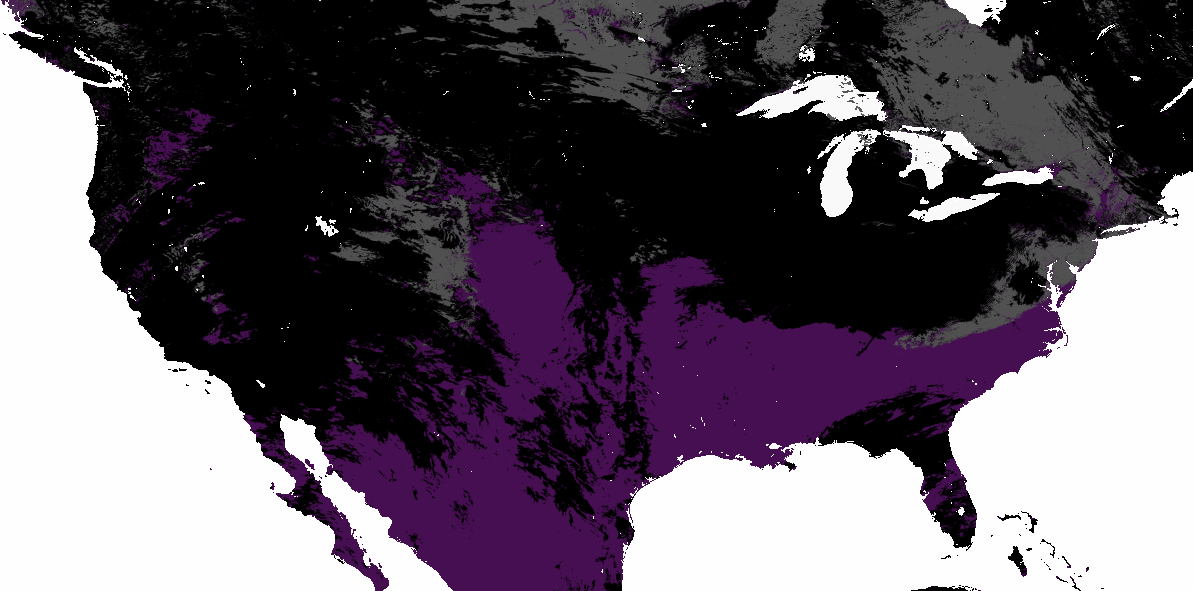
\includegraphics[width=0.23\textheight]{figs/newsat-12212009.png}} &
\fbox{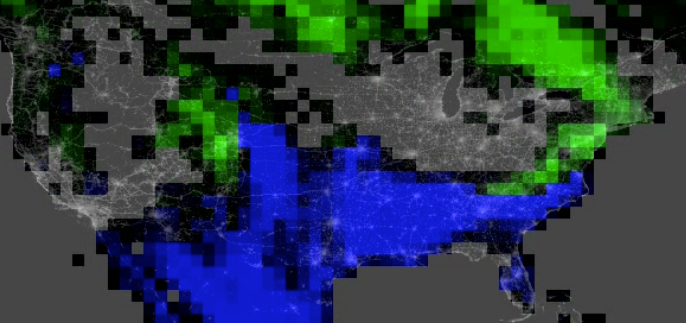
\includegraphics[width=0.23\textheight]{figs/sat-dec212009.png}} &
\fbox{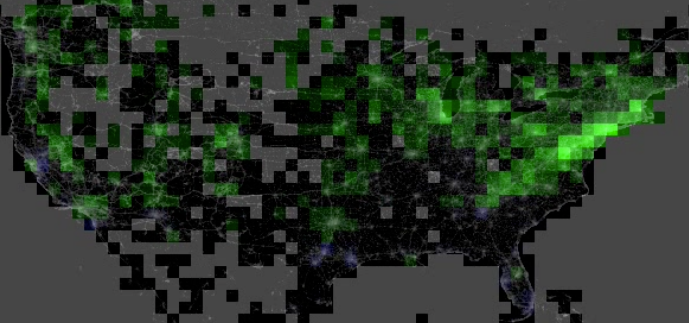
\includegraphics[width=0.23\textheight]{figs/flickr-dec212009.png}} \\
\end{tabular}
\end{center}
\vspace{-6pt}
\caption{Comparing MODIS satellite snow coverage data for North
  America on Dec 21, 2009 with estimates produced by analyzing Flickr
  tags (best viewed on screen in color). \textit{Left:} Original MODIS snow data, where white
  corresponds with water, black is missing data because of cloud
  cover, grey indicates snow cover, and purple indicates no
  significant snow cover.  \textit{Middle:} Satellite data coarsened
  into 1 degree bins, where green indicates snow cover, blue indicates
  no snow, and grey indicates missing data.  \textit{Right:} Estimates
  produced by the Flickr photo analysis proposed in this paper, where
  green indicates high probability of snow cover, and grey and black
  indicate low-confidence areas (with few photos or ambiguous evidence).}
\label{fig:samplemap}
\end{figure*}


Third, while ground truth is available for these particular
phenomena, for other important ecological phenomena (like the geo-temporal distribution of plants and animals) no such data is
available, and social media could help fill this need.
%, and mining data from social media has the potential to fill
%this gap.  
In fact, perhaps no community is in greater need of
real-time, global-scale information on the state of the world than the
scientists who study climate change. Recent work shows that global
climate change is impacting a variety of flora and fauna at local,
regional and continental scales: for example, species of
high-elevation and cold-weather mammals have moved northward, some
species of butterflies have become extinct, waterfowl are losing
coastal wetland habitats as oceans rise, and certain fish populations
are rapidly declining~\cite{ipcc2007climate}. However monitoring these
changes is surprisingly difficult: plot-based studies
involving direct observation of small patches of land yield
high-quality data but are costly and possible only at very small
scales, while aerial surveillance gives data over
large land areas but cloud cover, forests, atmospheric
conditions and mountain shadows can interfere with the observations,
and only certain types of ecological information can be collected from
the air.  To understand how biological phenomena are responding to
both landscape changes and global climate change, ecologists need an
efficient system for ground-based data collection to give detailed
observations across the planet.  A new approach
for creating ground-level, continental-scale datasets is to use
passive data-mining of the huge number of visual observations produced
by millions of users worldwide, in the form of digital images uploaded
to photo-sharing websites.


\xhdr{Challenges.}
There are two key challenges to unlocking the ecological
information latent in these photo datasets. The first is how to recognize 
ecological phenomena appearing in photos and how to map these observations to
specific places and times. Fortunately, modern photo-sharing sites
collect a rich variety of non-visual
information about photos, including metadata recorded by the digital
camera --- exposure settings and timestamps, for example --- as well as
information generated during social sharing  ---
text tags, comments, and ratings, for example. Many sites also
record the
 geographic coordinates of where on Earth a photo was taken, as reported either by a GPS-enabled camera or smartphone, or input manually by the user.
Thus online photos include the ingredients
necessary to produce geo-temporal data about the world,
including information about content (images, tags and comments), and
when (timestamp) and where (geotag) each photo was taken.

The second challenge is how to deal with the biases and noise inherent
in online data. People do not photograph the Earth evenly,
 so there are disproportionate concentrations of
activity near cities and tourist attractions. Photo metadata is often
noisy or inaccurate; for example, users forget to set the clock on
their camera, GPS units fail to find fixes, and users
carelessly tag photos.  Even photos without such errors might be
misleading: the tag ``snow'' on an image might refer to a snow lily or a
snowy owl, while snow appearing in an image might be artificial (as in an indoor zoo exhibit).

\xhdr{This paper.}  In this paper we study how to mine data from
photo-sharing websites to produce crowd-sourced observations of
ecological phenomena.  As a first step towards the longer-term goal of
mining for many types of phenomena, here we study two in particular:
ground snow cover and vegetation cover (``green-up'') data. Both are
critical features for ecologists monitoring the earth's ecosystems.
Importantly for our study, these two phenomena have accurate
fine-grained ground truth available at a continental scale in the form
of observations from aerial instruments like NASA's Terra earth-observing
satellites~\cite{modisveg,modissnow} or networks of ground-based
observing stations run by the U.S. National Weather Service. This
data allows us to evaluate the performance of our crowd-sourced data mining
techniques at a very large scale, including thousands of days of data
across an entire continent.
%This evaluation gives insight into how accurate crowd-sourced 
%observations could be for tracking ecological phenomena for which
%no ground truth exists.
 Using a dataset of nearly 150 million geo-tagged Flickr photos, we
 study whether this data can potentially be a
 reliable resource for scientific research.  An example comparing
 ground truth snow cover data with the estimates produced by our
 Flickr analysis on one particular day (December 21, 2009) is shown in
 Figure~\ref{fig:samplemap}. Note that the Flickr analysis is sparse
 in places with few photographs, while the satellite data is missing
 in areas with cloud cover, but they agree well in areas where both
 observations are present. This (and the much more extensive experimental results presented later in the paper) suggests that Flickr analysis may produce
 useful observations either on its own or as a complement other
 observational sources.


%% More generally, this paper is a step towards answering a more basic
%% question: How reliable could passive mining of social sharing sites be
%% in producing observations of the world?  Analyzing data from social
%% networking and microblogging websites to make estimations and
%% predictions about world events has become a popular research
%% direction, including for example tracking the spread of
%% disease~\cite{ginsberg09flu}, monitoring for fires and other
%% emergencies~\cite{delongueville09}, predicting product adoption and
%% election outcomes~\cite{jin10prediction}, and inferring aggregate
%% public mood~\cite{oconnor10mood,bollen11twitter}. In most of these
%% studies, however, there is either no ground truth to judge the quality
%% of the estimates, or the ground truth that is used is an indirect
%% proxy (e.g. since no aggregate public mood data exists,
%% \cite{oconnor10mood} evaluates against opinion polls,
%% while~\cite{bollen11twitter} compares to stock market indices). In
%% contrast, for predicting some ecological phenomena like vegetation and
%% snow cover, we have daily, dense ground-truth data for the entire
%% globe in the form of satellite observations.

To summarize, the main contributions of this paper include: 

\begin{packed_itemize}
\item[---] introducing the novel idea of mining photo-sharing sites for
  geo-temporal information about ecological phenomena, 
\item[---] introducing several techniques for deriving crowd-sourced
  observations from noisy, biased data using both visual and textual tag analysis, and
\item[---] evaluating the ability of these techniques to accurately measure
  these phenomena, using dense large-scale ground truth.
\end{packed_itemize}


\section{related work}

A variety of recent work has studied how to apply computational
techniques to analyze online social datasets in order to aid research
in other disciplines~\cite{lazer09}. Much of this work has studied
questions in sociology and human interaction, such as how friendships
form~\cite{feedback08kdd}, how information flows through social
networks~\cite{libennowell08}, how people move through
space~\cite{brockmann06}, and how people influence their
peers\cite{anagnostpopoulos08}.  The goal of these projects is not to
measure data about the physical world itself, but instead to discover
interesting properties of human behavior using social networking sites
as a convenient data source.

\xhdr{Crowd-sourced observational data.}
Other studies have shown the power of social networking sites as a
source of observational data about the world itself.  Bollen
\textit{et al}~\cite{bollen11twitter} use data from Twitter to try to measure
the aggregated emotional state of humanity, computing mood across six
dimensions according to a standard psychological
test. Intriguingly, they find that these changing mood states
correlate well with the Dow Jones Industrial Average, allowing stock
market moves to be predicted up to 3 days in advance.  However their
test dataset is relatively small, consisting of only three weeks of
trading data.  Like us, Jin~\textit{et al}~\cite{jin10prediction} use
Flickr as a source of data for prediction, but they estimate the
adoption rate of consumer photos by monitoring the frequency of tag
use over time. They find that the volume of Flickr tags is 
correlated  with with sales of two products, Macs and iPods. They also
estimate geo-temporal distributions of these sales over time but do
not compare to ground truth, so it is unclear how accurate these
estimates are. In contrast, we evaluate our techniques against a large
ground truth dataset, where the task is to accurately predict the
distribution of a phenomenon (e.g. snow) across an entire continent 
each day for several years.

\xhdr{Crowd-sourced geo-temporal data.}
Other work has used online data to predict geo-temporal distributions,
but again in domains other than ecology.  Perhaps the most
striking is the work of Ginsberg \textit{et al}~\cite{ginsberg09flu},
who show that by monitoring the geospatial distribution of search
engine queries related to flu symptoms, the spread of the H1N1
flu can be estimated several days before the official statistics produced by traditional
means.
DeLongueville \textit{et
  al}~\cite{delongueville09} study tweets related to a major fire in
France, but their analysis is at a very small scale (a few dozen
tweets) and their focus is more on human reactions to the fire as
opposed to using these tweets to estimate the fire's position and
severity.  In perhaps the most related existing work to ours,
 Singh \textit{et al}~\cite{singh10socialpixels} create
geospatial heat maps (dubbed ``social pixels'') of various
tags, including snow and greenery, but their focus is on developing a
formal database-style algebra for describing queries on these systems
and for creating visualizations. They do not consider how to produce
accurate predictions from these visualizations, nor do they compare to
any ground truth.

\xhdr{Citizen science.}
While some volunteer-based biology efforts like the Lost Ladybug
Project~\cite{lostladybug} and the Great Sunflower
Project~\cite{greatsunflower} use social networking sites to
organize and recruit volunteer observers, we are not aware of any
work that has attempted to passively mine ecological data from social media
sites. The visual data in online social networking sites provide a
unique resource for tracking biological phenomena:  because they are
images, this data can be verified in ways that simple text 
cannot.  In addition, the rapidly expanding quantity
of online images with geo-spatial and temporal metadata creates a
fine-scale record of what is happening across the globe.  However, to
unlock the latent information in these vast photo collections, we need
 mining and recognition tools that can efficiently
process large numbers of images, and robust statistical models that
can handle incomplete and incorrect observations.

\section{Our approach}

%\subsection{Datasets}

We use a sample of nearly 150 million geo-tagged, timestamped Flickr
photos as our source of user-contributed observational data about the
world. We collected this data using the public Flickr API, by
repeatedly searching for photos within random time periods and
geo-spatial regions, until the entire globe and all days between January 1, 2007 and December 31, 2010 had been covered.
We applied filters to remove blatantly inaccurate
metadata, in particular removing photos with geotag precision less
than about city-scale (as reported by Flickr), and photos whose upload
timestamp is the same as the EXIF camera timestamp (which usually
means that the camera timestamp was missing).  

For ground truth we use large-scale data originating from two
independent sources: ground-based weather stations, and aerial
observations from satellites.  For the ground-based observations, we
use publicly-available daily snowfall and snow depth observations from
the U.S. National Oceanic and Atmospheric Administration (NOAA) Global
Climate Observing System Surface Network (GSN)~\cite{ghcn}.  This data
provides highly accurate daily data, but only at sites that have
surface observing stations. 
%
For denser, more global coverage, we also use
data from the Moderate Resolution Imaging Spectroradiometer (MODIS)
instrument aboard NASA's Terra satellite. The satellite is in a polar
orbit so that it scans the entire surface of the earth every day. The
MODIS instrument measures spectral emissions at various wavelengths,
and then post-processing uses these measurements to estimate ground cover.
In this paper we use two datasets: the daily snow cover
maps~\cite{modissnow} and the two-week vegetation
averages~\cite{modisveg}. Both of these sets of data including an
estimate of the percentage of snow or vegetation ground cover at each
point on earth, along with a quality score indicating the confidence
in the estimate. Low confidence is caused primarily by cloud cover
(which changes the spectral emissions and prevents accurate ground
cover from being estimated), but also by technical problems with the
satellite. 
As an example, Figure~\ref{fig:samplemap} shows raw satellite snow data from one particular day.




%% \begin{figure}
%% \begin{center}
%% \begin{tabular}{cc}
%% 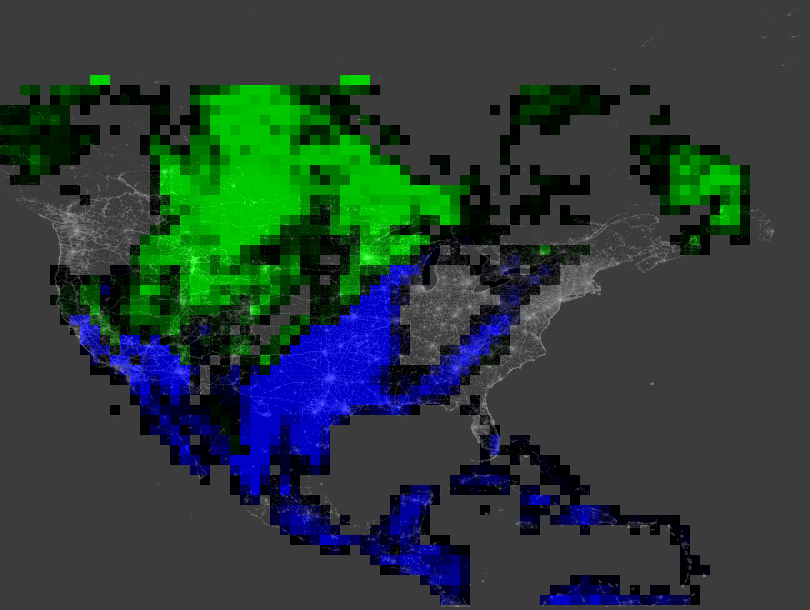
\includegraphics[width=0.5\textwidth]{plots/nasadownsample20070101.png}
%% \end{tabular}
%% \end{center}
%% \caption{Down-sampled NASA MODIS snow coverage data for North America
%%   on 2007.01.01. Grey: water-covered, or no data, or the confidence
%%   index value is 0; blue: no snow and has non-zero confidence index
%%   value; green: has snow and non-zero confidence index value. (Please
%%   view in color.)}
%% \label{fig:nasadownsample20070101}
%% \end{figure}


\subsection{Estimation techniques}
\label{sec:methods}

Our goal is to estimate the presence or absence of a given ecological
phenomenon (like a species of plant or flower, or a meteorological
feature like snow) on a given day and at a given place,
using only the geo-tagged, time-stamped photos from Flickr. One way of viewing
this problem is that every time a user takes a photo of a phenomenon
of interest, they are casting a ``vote''  that the
phenomenon actually occurred in a given geospatial region. 
 We could
simply look for tags indicating the presence of a feature --
i.e. count the number of photos with the tag ``snow'' --  
but sources of noise and bias make this task 
challenging, including:
\begin{packed_itemize}
\item[---] \textit{Sparse sampling:} The geospatial distribution of photos
  is highly non-uniform. A lack of photos
  of a phenomenon in a region does not
  necessarily mean that it was not there. 
\item[---] \textit{Observer bias:} Social media users are younger and
  wealthier than average, and most live in North
  America and Europe.
\item[---] \textit{Incorrect, incomplete and misleading tags:}
  Photographers may use incorrect or ambiguous tags  ---
  e.g. the tag ``snow'' may refer to a snowy owl or interference on a
  TV screen.
\item[---] \textit{Measurement errors:} Geo-tags and timestamps are
  often incorrect (e.g. because people   forget to set their camera clocks).
\end{packed_itemize}

\xhdr{A statistical test.}  We introduce a simple probabilistic model
and use it to derive a statistical test that can deal with some such
sources of noise and bias. The test could be used for estimating the
presence of any phenomenon of interest; without loss of generality we
use the particular case of snow here, for ease of explanation.  Any
given photo either contains evidence of snow (event $s$) or does not
contain evidence of snow (event $\bar{s}$).  We assume that a given
photo taken at a time and place with snow has a fixed probability $P(s
| snow)$ of containing evidence of snow; this probability is less than
1.0 because many photos are taken indoors, and outdoor photos might be
composed in such a way that no snow is visible. We also assume that
photos taken at a time and place without snow have some non-zero
probability $P(s | \overline{snow})$ of containing evidence of snow;
this incorporates various scenarios including incorrect timestamps or
geo-tags and misleading visual evidence (e.g.  man-made
snow).

Let $m$ be the number of snow
photos (event $s$), and $n$ be the number of non-snow photos (event
$\bar{s}$) taken at a place and time of interest. Assuming that each photo is captured
independently, we can use Bayes' Law to
derive the probability that a given place has snow
given its number of snow and non-snow photos,
%
%\newcommand{\smsn}{\overbrace{s\cdots s}^{m},\overbrace{\overline{s}\cdots \overline{s}}^{n}}
%%hp cr: \bar{s}^n
\newcommand{\smsn}{s^m, \bar{s}^n}
\newcommand{\smsntwo}{s^m, \bar{s}^n}
%%\newcommand{\smsn}{s^m, s^n}
%%\newcommand{\smsntwo}{s^m, s^n}
%\newcommand{\smsntwo}{\underbrace{s\cdots s}_{m},\underbrace{\overline{s}\cdots \overline{s}}_{n}}
\begin{eqnarray*}
P(snow|\smsn)  &=&\frac{ P(\smsn|snow)P(snow)}{P(\smsntwo)}  \\
&=&\frac{{m+n\choose m}p^{m}(1-p)^{n}P(snow)}{P(\smsntwo)},  
\end{eqnarray*}
%
where we write $s^m, \bar{s}^n$ to denote $m$ occurrences of event $s$ and $n$ occurrences of event $\bar{s}$, and where $p=P(s|snow)$ and $P(snow)$ is the prior probability of snow. A similar derivation gives the posterior probability that the bin does not contain snow,
%
\begin{eqnarray*}
P(\overline{snow}|\smsn)  &=&\frac{{m+n\choose m}q^{m}(1-q)^{n}P(\overline{snow})}{P(\smsntwo)},  
\end{eqnarray*}
%
where $q=P(s|\overline{snow})$. 
%
Taking the ratio between these two posterior probabilities yields a likelihood ratio,
%
\begin{eqnarray}
\frac{P(snow|\smsn)}{P(\overline{snow}|\smsntwo)}
%\\=\frac{\frac{{m+n\choose m}p^{m}(1-p)^{n}P(snow)}{P(\overbrace{s\cdots s}^{m},\overbrace{\overline{s}\cdots \overline{s}}^{n})}}{\frac{{m+n\choose m}q^{m}(1-q)^{n}P(\overline{snow})}{P(\overbrace{s\cdots s}^{m},\overbrace{\overline{s}\cdots \overline{s}}^{n})}}
&=&\frac{P(snow)}{P(\overline{snow})}\left(\frac{p}{q}\right)^{m}\left(\frac{1-p}{1-q}\right)^n.
\label{eq:conf}
\end{eqnarray}
%
This ratio can be thought of as a measure of the confidence that a
given time and place actually had snow, given photos from Flickr.

A simple way of classifying a photo into a positive event $s$ or a
negative event $\bar{s}$ is to use text tags. We identify a
set ${\cal S}$ of tags related to a phenomenon of
interest. Any photo tagged with at least one tag in ${\cal S}$ is
declared to be a positive event $s$, and otherwise it is considered a
negative event $\bar{s}$. For the snow detection task, we use the set
${\cal S}$=\{snow, snowy, snowing, snowstorm\}, which we selected
by hand.

%%, which we chose by
%%looking at the 200 most frequent Flickr tags and hand selecting those
%%directly relevant to snowfall.

The above derivation assumes that photos are taken independently of
one another, which is generally not true in reality. One particular
source of dependency is that photos from the same user are highly
correlated with one another.  To mitigate this problem, instead of
counting $m$ and $n$ as numbers of \textit{photos}, we instead let $m$ be 
the number of \textit{photographers} having at least one photo with evidence of snow,
while $n$ is the numbers of photographers who did not upload any
photos with evidence of snow.

The probability parameters in the likelihood ratio of
equation~(\ref{eq:conf}) can be directly estimated from training data
and ground truth. For example, for the snow cover results
presented in Section~\ref{sec:results}, the learned parameters are: $p
= p(s|snow) = 17.12\%$, $q = p(s|\overline{snow}) = 0.14\%$.  In other
words, almost 1 of 5 people at a snowy place take a photo containing
snow, whereas about 1 in 700 people take a photo containing evidence
of snow at a non-snowy place.

Figure~\ref{fig:samplemap} shows a visualization of the likelihood
ratio values for the U.S. on one particular day using this simple
technique with ${\cal S}$=\{snow, snowy, snowing, snowstorm\}.  High
likelihood ratio values are plotted
in green, indicating a high confidence of snow in a geospatial bin,
while low values are shown in blue and indicate high confidence of 
no snow.  Black areas indicate a likelihood ratio 
near 1, showing little conference either way, and grey areas lack
data entirely (having no Flickr photos in that bin on that day).

\subsection{Learning features automatically}

The confidence score in the last section has a number of limitations,
including requiring that a set of tags related to the phenomenon of
interest be selected by hand. Moreover, it makes no attempt to
incorporate visual evidence or negative textual evidence --- e.g.,
that a photo tagged ``snowy owl'' probably contains a bird and no
actual snow.  We use machine learning techniques to address these
weaknesses, both to automatically identify specific tags and tag
combinations that are correlated with the presence of a phenomenon of
interest, and to incorporate visual evidence into the prediction techniques.

\xhdr{Learning tags.}  We consider two learning paradigms. The first
is to produce a single exemplar for each bin in time and space
consisting of the set of all tags used by all users. For each of these
exemplars, the NASA and/or NOAA ground truth data gives a label (snow
or non-snow). We then use standard machine learning algorithms like
Support Vector Machines and decision trees to identify the most
discriminative tags and tag combinations. In the second paradigm, our
goal instead is to classify individual \textit{photos} as containing
snow or not, and then use these classifier outputs to compute the
number of positive and non-positive photos in each bin (i.e., to
compute $m$ and $n$ in the likelihood ratio described in the last
section).

\xhdr{Learning visual features.}  We also wish to incorporate visual
evidence from the photos themselves. There is decades of
work in the computer vision community on object and scene
classification (see~\cite{szeliski} for a recent survey), although
most of that work has not considered the large, noisy photo collections we work with here. We tried a number of
approaches, and found that a classifier using a simplified version of
GIST  augmented with color features~\cite{gist, hays}
gave a good trade-off between accuracy and 
tractability.

\newcommand{\lab}{CIELAB }
Given an image $I$, we partition the image into a $4 \times 4$ grid of
16 equally-sized rectangular regions. In each region we compute the
average pixel values in each of the red, green, and blue color planes,
and then convert this color triple from sRGB space to the \lab color
space~\cite{lab}. \lab  has a number of advantages, including
separating greyscale intensity from the color channels and having greater
perceptual uniformity (so that Euclidean distances between two \lab
color triples are approximately proportional to the human perception
of difference between the colors). For each region $R$ we also compute the
total gradient energy $E(R)$ within the grayscale plane $I_g$ of the image,
%
\begin{eqnarray*}
E(R) & = & \sum_{(x,y) \in R}   || \nabla I_g(x,y) || \\
& = & \sum_{(x,y) \in R} \sqrt{I_x(x,y)^2 + I_y(x,y)^2}, 
\end{eqnarray*}
%
where $I_x(x,y)$ and $I_y(x,y)$ are the partial derivatives in the $x$
and $y$ directions evaluated at point $(x,y)$, approximated as,
%
\begin{eqnarray*}
I_x(x,y) = I_g(x+1, y) - I_g(x-1, y), \\
 I_y(x,y) = I_g(x, y+1) - I_g(x, y-1).
\end{eqnarray*}
%
  For each image we
concatenate the gradient energy in each of the 16 bins, followed by
the 48 color features (average L, a, and b values for each of the 16
bins), to produce a 64-dimensional feature vector.  We then learn a
Support Vector Machine (SVM) classifier from a labeled training image
set.

\section{Experiments and results}
\label{sec:results}

We now turn to presenting experimental results for estimating the
geo-temporal distributions of two ecological phenomena: snow and vegetation cover.
In addition to the likelihood ratio-based score described in
Section~\ref{sec:results} and machine learning approaches, we also
compare to two simpler techniques: \textit{voting,} in which 
we simply count the number of users that use one of a set
$S$ of tags related to the phenomenon of interest at a given time and place, and
\textit{percentage,} in which we calculate the ratio of users that use
one of the tags in $S$ over the total number of users who took a photo
in that place on that day.

\subsection{Snow prediction in cities}

%%%%%%%%%%%%%%%%%%%%%%
% hz added this for ROC curves
%We convert this problem to a binary prediction problem to compare different method with ROC curves. For each method, we slide a threshold for the bins that have photos. Predictions will be made only for the bins with ground truth and photos for which snow bins are positive cases and non-snow bins are negative cases.
%The confidence method and percentage method have single values to threshold while for voting method, we split it into two, as it has snow voters and no-snow voters. To make predictions using number of no-snow voters, we require the number of snow voters to be zero, while we don't consider the number of no-snow voters when using snow voters as thresholding values to make predictions. The baseline TPR for confidence, percentage and snow-voter voting is 2.76\%. % or 97.24%?
%and the baseline TPR for no-snow voter is 1.90\% (is it useful to use no-snow voter number to predict snow?)

%baseline_positive/baseline_total:0.0275996280425

% We first consider 

% \section{NOAA dataset}


We first test how well the Flickr data can predict snowfall at a local
level, and in particular for cities in which high-quality
surface-based snowfall observations exist and for which photo density is high.
%
%% We want to use it as a complete and reliable ground truth of daily
%% snow presence for major US cities where the Flickr user population is
%% also dense, such that we are able to train and test on the NOAA and
%% Flickr dataset to predict snow presence and even quantify it for every
%% day.
%
We choose 4 U.S. metropolitan areas, New York City, Boston, Chicago and
Philadelphia, and try to predict both daily snow presence as well as
the quantity of snowfall.  For each city, we define a corresponding
geospatial bounding box and select the NOAA ground observation stations in that area. 
For example, 
Figure~\ref{tab:city_statistics} shows the the stations 
and the bounding box for 
New York City. We calculate the ground truth daily snow quantity for a city as the average of
the valid 
snowfall values from its stations.
%, with the
%daily snow depth value obtained in a similar way. 
%% According to the
%% Climatological Data Publications
%% (http://www7.ncdc.noaa.gov/IPS/cd/cd.html) that are generated from
%% GHCN-Daily, the snowfall values reflect snowfall from 0 to 24 local
%% time daily in millimeters while the snow depth values are recorded
%% once at 12 UTC (GMT). So the snowfall after 12 UTC (GMT) that day is
%% not reflected by the snow depth value for that day. So we decide to
%% take the max value between the snowfall value and snow depth value as
%% an estimation of the quantity of snow presence on a particular day and
%% we call this value max\_snow.
We call any day with a non-zero snowfall or snowcover to be a snow day,
and any other day to be a non-snow day.
%and make binary snow presence predictions, we need to define ground
%truth snow and non-snow days: we let  days with max\_snow greater than 0
%be snow days and the rest be non-snow
%days. 
Figure~\ref{tab:city_statistics} also presents some basic statistics for
these 4 cities.  All of our experiments involve 4 years (1461 days) of
data from January 2007 through December 2010; we reserve the first two
years for training and validation, and the second two years for
testing.

%<<<<<<< .mine
%=======
%We choose 4 major cities in the US - New York City, Boston, Chicago
%and Philadelphia to predict their daily snow presence and the quantity
%of snow presence.  For each city, we choose a corresponding geo area
%and a list of reliable stations in that area defined and chosen by the
%Climatological Data Publications. In fig
%Figure~\ref{fig:nyc_stations}, we mark the stations we collect data
%from and the bounding box for selecting geostamped Flickr photos for
%New York City. The daily snowfall for a certain city is the average of
%the valid snowfall values from the stations in the defined area. The
%daily snow depth value is obtained in a similar way. 

%% According to the
%% Climatological Data Publications
%% ~\cite{noaa2} %(http://www7.ncdc.noaa.gov/IPS/cd/cd.html) that are
%% generated from GHCN-Daily, the snowfall values reflect snowfall from 0
%% to 24 local time daily in millimeters while the snow depth values are
%% recorded once at 12 UTC (GMT). So the snowfall after 12 UTC (GMT) that
%% day is not reflected by the snow depth value for that day. So we
%% decide to take the max value between the snowfall value and snow depth
%% value as an estimation of the quantity of snow presence on a
%% particular day and we call this value max\_snow.  In order to compute
%% Flickr confidence and make binary snow presence predictions, we need
%% to define ground truth snow and non-snow days. The days with max\_snow
%% greater than 0 are snow days and the days with max\_snow equal to 0
%% are non-snow days. Table~\ref{tab:city_statistics} shows some basic
%% statistics of the 4 cities.


\begin{figure}
\begin{center}
%\begin{tabular}{c}
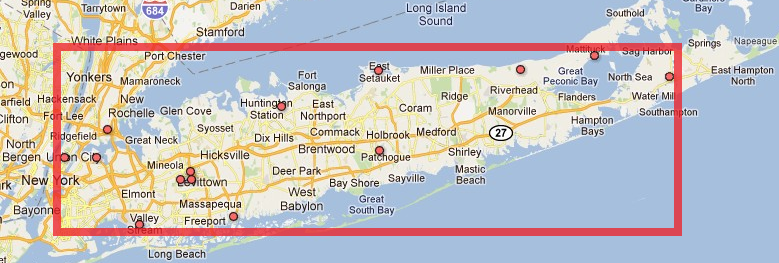
\includegraphics[width=0.35\textwidth]{plots/nyc_stations.png} 
%\end{tabular}
\end{center}
%\caption{New York City geospatial bounding box used to select Flickr photos, and locations of NOAA observation stations.}
%\label{fig:nyc_stations}
%\end{figure}
%
%
%
%\begin{table} 
% \caption {\textbf{Statistics about spatial area, photo density, and ground truth for each of the 4 cities.}}
%\label{tab:city_statistics} 
\begin{center}
{\small{
\newcommand{\spc}{\hspace{2pt}}
\begin{tabular} {|@{\spc}l@{\spc}|@{\spc}r@{\spc}|@{\spc}r@{\spc}|@{\spc}r@{\spc}|@{\spc}r@{\spc}|} 
\hline 
\textbf{} &{NYC}  &{Chicago} &{Boston}&{Philadelphia} \tabularnewline
\hline 
{Mean active Flickr users / day} &{65.6} &{94.9} &{59.7} &{43.7} \tabularnewline
\hline 
{Approx. city area ($km^2$)} &{3,712} &{11,584} &{11,456} &{9,472}  \tabularnewline
\hline 
{User density (avg users/unit area)} &{112.4} &{52.5} &{33.5} &{29.6} \tabularnewline
\hline 
{Mean daily snow (inches)} &{0.28} &{0.82} &{0.70} &{0.35} \tabularnewline
\hline 
{Snow days (snow>0 inches)} &{185} &{418} &{373} &{280} \tabularnewline
\hline 
{Number of obs. stations} &{14} &{20} &{41} &{26} \tabularnewline
\hline 
\end{tabular}}}
\end{center}
\vspace{-12pt}
 \caption {\textit{Top:} New York City geospatial bounding box used to select Flickr photos, and locations of NOAA observation stations. \textit{Bottom:} Statistics about spatial area, photo density, and ground truth for each of the 4 cities.}
\label{tab:city_statistics} 
\end{figure}

\xhdr{Daily snow classification for 4 cities.}
Figure~\ref{fig:city_roc}(a) presents ROC curves for this
daily snow versus non-snow classification task on New York City. The figure compares the likelihood
ratio confidence score from equation~(\ref{eq:conf}) to the baseline
approaches (voting and percentage), using the tag set
${\cal S}$=\{snow, snowy, snowing, snowstorm\}.
%%hp cr: added auc and p-values here and cited the paper.
The area under the ROC curve (AUC) statistics are 0.929, 0.905, and 0.903 for confidence, percentage, and voting, respectively, 
and the improvement of the confidence method is statistically significant 
with $p=0.0713$ according to the statistical test of~\cite{auc}.
%% The figure shows that the
%%confidence method has a better overall performance for NYC; it also
The confidence method also outperforms other methods for the other three cities (not shown due to
space constraints).  ROC curves for all 4 cities using the likelihood
scores are shown in Figure~\ref{fig:city_roc}(b). Chicago has the best
performance and Philadelphia has the worst; a possible explanation
is that Chicago has the most active Flickr users per
%%hp cr: changed 29.6 to 43.7
day (94.9) while Philadelphia has the least (43.7).
%%day (94.9) while Philadelphia has the least (29.6).

%here goes ML methods
%<<<<<<< .mine
These methods based on presence or absence of tags are simple and very
fast, but they have a number of disadvantages, including that the tag
set must be manually chosen and that negative correlations between
tags and phenomena are not considered.
We thus tried training a classifier to learn these relationships automatically.
For each day in each city, we produce a single binary feature vector indicating whether 
or not a given tag was used on that day. We also tried a feature selection step
by computing information gain and rejecting features below a threshold, as well as adding the likelihood score from equation~(\ref{eq:conf}) as an additional feature.
For all experiments we used feature vectors from 2007 and 2008 for training and tested on data from 2009 and 2010,
and used   
a LibLinear classifier with L2-regularized logistic regression~\cite{Fan2008}.
Table~\ref{tab:classifiers_snowcities} presents the results, showing that information gain
(IG) and confidence scores (Conf) improve the results for all cities,
and that the classifier built with both IG and Conf generally outperforms
other classifiers, except for Boston.
Figure~\ref{fig:city_roc}(c) shows 
ROC curves from different classifiers for NYC and
Figure~\ref{fig:city_roc}(d) compares ROC curves for the 4 cities
using the classifier using both feature selection and confidence. 
Note that the machine learning-based techniques substantially outperform the
simple likelihood ratio approach (compare
Figures~\ref{fig:city_roc}(b)  and
(d)).


%=======
%Meanwhile, we try machine learning methods with LibLinear classifier ~\cite{Fan2008} to solve this problem as well. For each city, we build a basic classifier based on the tags used by users each day. Besides using tags only as features, we use information gain to reduce the features space and confidence scores as an additional feature which proves to be a helpful feature. Training and testing data are divided in the same way (first half training and second half testing) as the confidence method. Table ~\ref{tab:classifiers_snowcities} 
%shows that information gain (IG) and confidence scores (Conf.) improve the results for all cities and the classifier built with both IG and Conf. generally outperform other classifiers, except for Boston, where
%the classifier with Conf. performs slightly better. Figure~\ref{fig:city_roc}(c) shows the comparisons of ROC curves from different classifiers for NYC and Figure~\ref{fig:city_roc}(d) compares ROC curves for the 4 cities using the classifier with IG and Conf. ROC curves in Figure~\ref{fig:city_roc}(d) are better than their counterparts in Figure~\ref{fig:city_roc}(b).
%>>>>>>> .r1762
%mk i added the follwoing sentence to show the improvement over the baseline
%In Regression case we have margin imporovement for binary prediction between 3% and 10.8%
% while in classification we have margin imporovement between 8% and 22.5%
%By using the classifier with IG and Conf., we achieve (16.2 \%,22.5,\%,8\% and 12.2 \%)   improvements than the baseline for (Boston, Chicago,NYC and Philadelphia ) respectively.
%Baseline is shown in the ROC curve figures. The percentages are not important.

%question about the table for binary ML, why accuracy and recall have the same values? 
% They should be the same.  

%should we mention regression is much faster?
% i think  the difference in computation between classifier and regression is clear. i think we don't need to mention anything about that.
 
\begin{table}[b!] 
 \caption {\textbf{ Daily snow clasification results for a 2 year period (2009--2010) for four major metropolitan areas.}}
\label{tab:classifiers_snowcities} 
\begin{center}
{\small{
\newcommand{\spc}{\hspace{2pt}}
\begin{tabular} {|@{\spc}c@{\spc}|@{\spc}c@{\spc}|@{\spc}c@{\spc}|@{\spc}c@{\spc}|@{\spc}c@{\spc}|@{\spc}c@{\spc}|} %{| \spa  r \spa | *{4}{\spa l \spa|}}   %{@{}c@{}c@{}c@{}c@{}c@{}}
\hline 
   %&   &  \textbf{\#}     %\tabularnewline
 \textbf{Features} & \textbf{Accuracy}  &  \textbf{Precision} & \textbf{Recall}&  \textbf{F-Measure}  &\textbf{Baseline} \tabularnewline
%\hline
\hline 
%
\multicolumn{6}{|c|}{\textbf{NYC} } \\ %\tabularnewline
\hline
\textbf{Tags} & 0.859  &     0.851 &    0.859 &    0.805 &0.85 \\   % \tabularnewline
\hline 
\textbf{Tags+Conf.} &0.926 &   0.927 &    0.926   &  0.917 &0.85\\ %  \tabularnewline
\hline
\textbf{Tags+IG} & 0.91   &    0.906 &    0.91  &    0.898 &0.85  \\ % \tabularnewline
\hline 
\textbf{Tags+IG+Conf.}& \textbf{0.93}   & \textbf{ 0.93}  &  \textbf{  0.93}  &  \textbf{  0.923} &\textbf{0.85}  \\ % \tabularnewline

\hline
 \multicolumn{6}{|c|}{\textbf{Boston}}  \\ %\tabularnewline
\hline

 \textbf{Tags} &0.899 & 0.897  & 0.899  &   0.894  & 0.756  \\   % \tabularnewline
\hline 
\textbf{Tags+Conf.} &\textbf{0.93}  &\textbf{ 0.929}  &  \textbf{ 0.93} & \textbf{0.929} &\textbf{0.756} \\ %  \tabularnewline
\hline
\textbf{Tags+IG} &  0.91    &   0.911  &   0.91 &     0.91 &0.756  \\ % \tabularnewline
\hline 
\textbf{Tags+IG+Conf.} & 0.923     &   0.923   &  0.923  &   0.923 &0.756 \\ % \tabularnewline
\hline 

 \multicolumn{6}{|c|}{\textbf{Chicago}}  \\ %\tabularnewline
\hline
\textbf{Tags} &0.937  & 0.938&     0.937 &    0.935 &0.728 \\   % \tabularnewline
\hline 
\textbf{Tags+Conf.} &0.949 &       0.952  &   0.949 &    0.948 &0.728  \\ %  \tabularnewline
\hline
\textbf{Tags+IG} &  0.938  &  0.938 &    0.938   &  0.938 &0.728 \\ % \tabularnewline
\hline 
\textbf{Tags+IG+Conf.} & \textbf{0.953}  & \textbf{0.954}  & \textbf{0.953}  & \textbf{0.953}  &\textbf{0.728} \\ % \tabularnewline


\hline 

\multicolumn{6}{|c|}{\textbf{Philadelphia}}  \\ %\tabularnewline
\hline
\textbf{Tags} & 0.849   &  0.851  &   0.849 &    0.815 &0.805  \\   % \tabularnewline
\hline 
\textbf{Tags+Conf.} &0.912   &   0.917  &   0.912 &    0.903 &0.805 \\ %  \tabularnewline
\hline
\textbf{Tags+IG} & 0.903    &   0.899 &    0.903 &    0.897 &0.805  \\ % \tabularnewline
\hline 
\textbf{Tags+IG+Conf.}& \textbf{0.927}    & \textbf{0.926} & \textbf{ 0.927} &  \textbf{0.924} &\textbf{0.805}    \\ % \tabularnewline
\hline 
\end{tabular}}}
\end{center}
\end{table}

%The following figures are NOT REFERRED anywhere, need to be replaced by figures mentioned in text above.
%%%%%%%%%%%%ML ROC for NOAA data set Cities (Boston-Chicago-NYC-Philly)
%\begin{figure*}
%\begin{center}
%\begin{tabular}{|@{}c@{}|@{}c@{}|@{}c@{}|@{}c@{}|}
%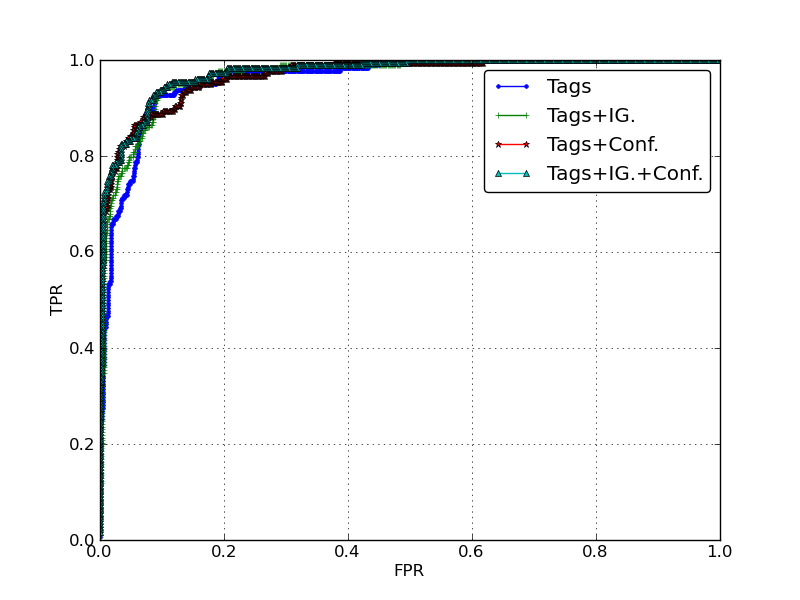
\includegraphics[width=0.25\textwidth]{plots/boston_LibLinear_Tag-Info-Cong-TagInfoConf.png} &
%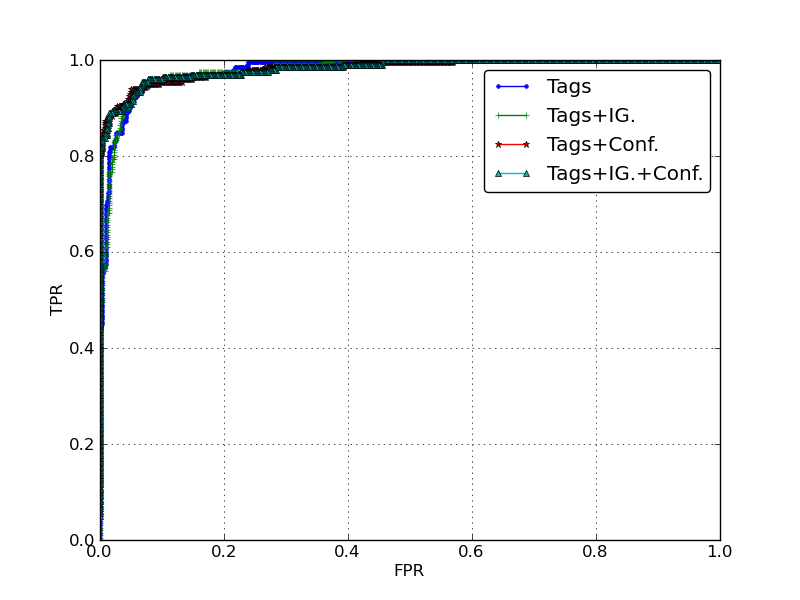
\includegraphics[width=0.25\textwidth]{plots/chicago_LibLinear_Tag-Info-Cong-TagInfoConf.png} &
%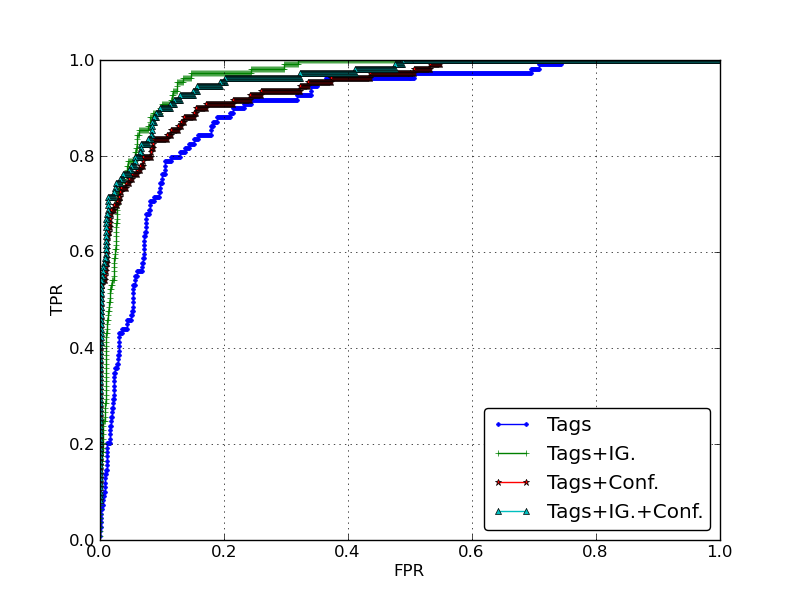
\includegraphics[width=0.25\textwidth]{plots/nyc_LibLinear_Tag-Info-Cong-TagInfoConf.png} &
%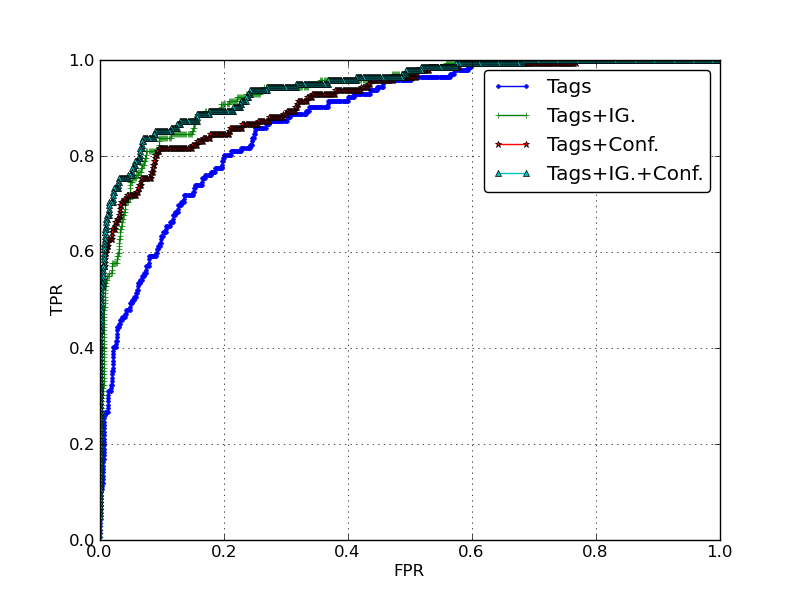
\includegraphics[width=0.25\textwidth]{plots/philly_LibLinear_Tag-Info-Cong-TagInfoConf.png} \\
%(a) & (b) &(c) & (d)  \\
%\end{tabular}
%\end{center}
%\caption{ROC Performance curves from LibLinear classifier, using NOAA dataset for snow vs. non-snow  classification: (a) Boston, (b) Chicago, (c)NYC  and (d) Philadelphia}
%\label{fig:classifier_for_each_city}
%\end{figure*}


%\xhdr{Daily quantified snow presence predictions for 4 cities.}
%To classify snow  vs. non-snow days,  we used   a binary classifier (LibLinear) ~\cite{Fan2008}. 
%we build classifier based on the tags used by users for each day. Beside using tags only as features  we used information gain to reduce the features space and  scored from the confidence method. For each city we used first two year's (2007-2008) for building model and second two year's(2009-2010) to evaluate the model.  Results in  ~\ref{tab:classifiers_snowcities} shows that both information gain and confidence scores improve the results for all cities. Basic classifier based on tags only working better than base-line for all cities. Base-line in this case is to predict all  as the majority class. By using the information gain and confidence, we are able to achieve (16.2 \%,22.5,\%,8\% and 12.2 \%)   improvement than the baseline for (Boston, Chicago
%NYC and Philadelphia ) respectively. 

\begin{figure*}
%\begin{center}
\hspace{-0.25in}
\small{
\begin{tabular}{@{}c@{}c@{}c@{}c@{}}
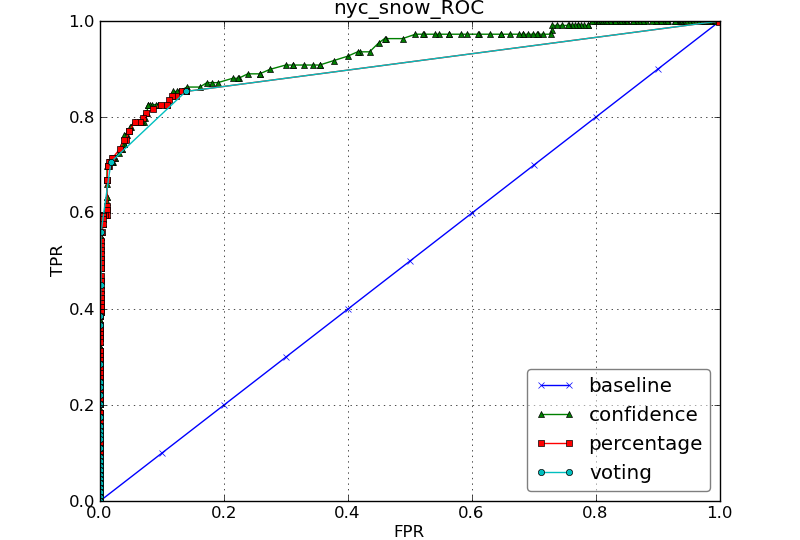
\includegraphics[width=0.255\textwidth,clip,trim=0.4in 0 0.8in 0]{plots/nyc_snow_ROC.png} &
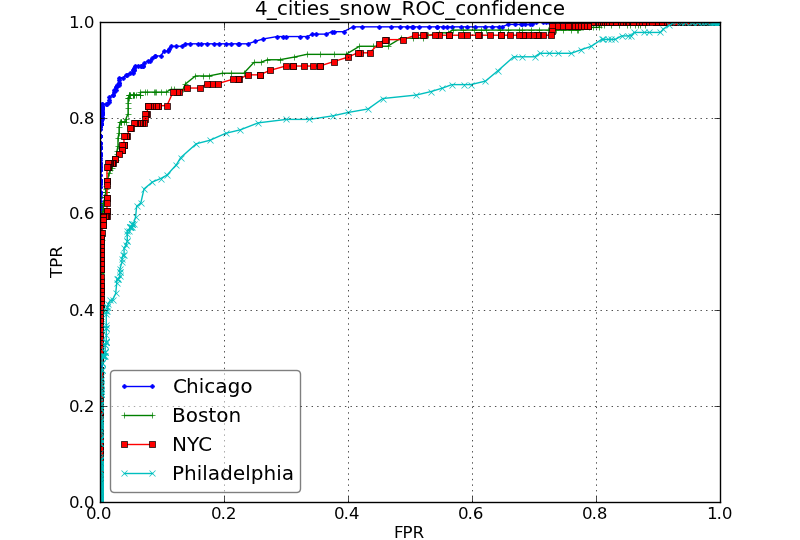
\includegraphics[width=0.255\textwidth,clip,trim=0.4in 0 0.8in 0]{plots/city_cmp_snow_ROC.png} &
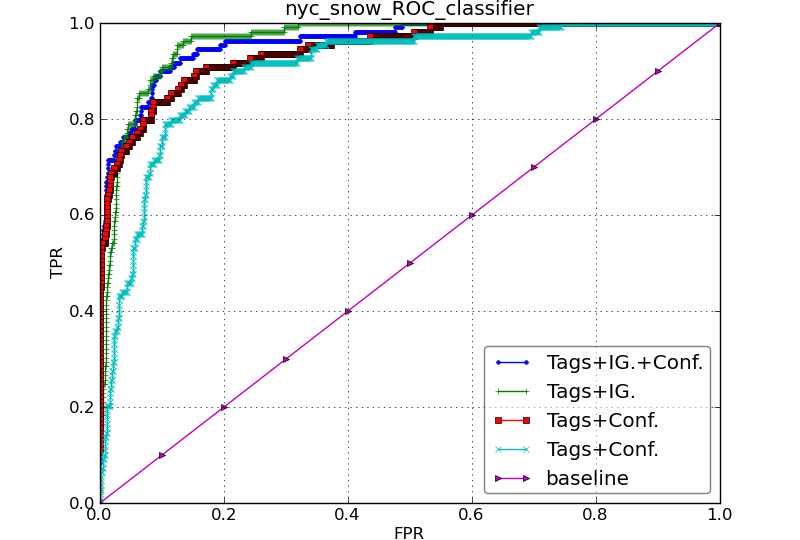
\includegraphics[width=0.255\textwidth,clip,trim=0.4in 0 0.8in 0]{plots/nyc_LibLinear_Tag-Info-conf-TagInfoConf_baseline.png} &
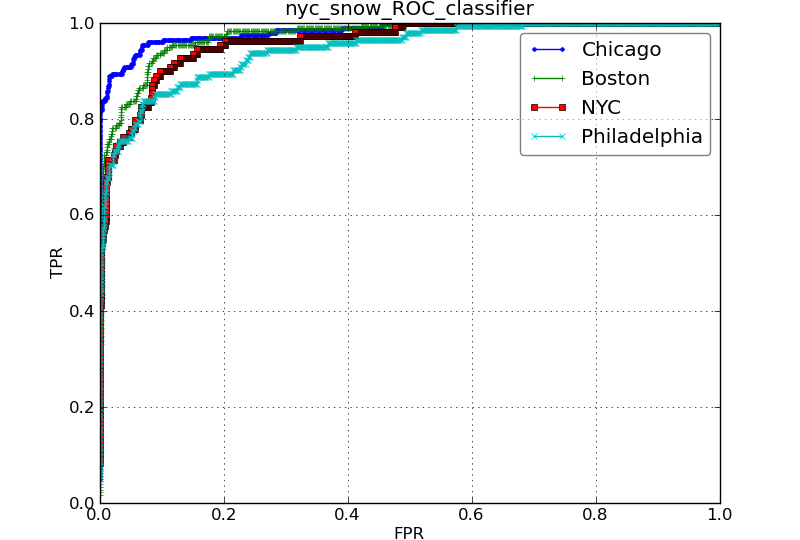
\includegraphics[width=0.255\textwidth,clip,trim=0.4in 0 0.8in 0]{plots/ROC_4cities_Tags_conf_info.png} \\
(a) & (b)  & (c) & (d) 
\end{tabular}
}
%\end{center}
\vspace{-6pt}
\caption{ROC curves for binary snow predictions: (a) ROC curves for New York City, comparing likelihood
ratio confidence score to voting and percentage approaches, (b) ROC curves for 4 cities using the likelihood
scores, (c)  ROC curves from SVM classifiers with different features for New York City, and (d) ROC curves for 4 cities using the logistic regression (LibLinear)
classifier with tags, information gain and confidence features. (Best viewed in color.)}
\label{fig:city_roc}
\vspace{-6pt}
\end{figure*}

\xhdr{Predicting snow quantities.}
In addition to predicting simple presence or absence of a phenomenon, it may be possible to predict the degree or quantity of that phenomenon. Here we try one particular approach, 
using our observation that the 
numerical likelihood score of equation~(\ref{eq:conf}) is somewhat correlated with depth of snow 
($R^2$=0.2972) --- i.e., that people take more photos of more severe storms (see Figure~\ref{fig:nyc_daily_conf_maxsnow}).
%
%shows the daily max\_snow
%values and confidence values for NYC which suggests a correlation
%between them. We also plot the days on which confidence and max\_snow
%values are both greater than 0 on both normal scale and log scale in
%Figure~\ref{fig:confidence_vs_maxsnow}. The latter suggests a possible
%linear relationship as it spreads out the data points. 
%A least-squares linear regression fit between the confidence score and
%actual snow amount has a 
%$p$-value of 4.933e-11 and an R-square of
%0.2972.
%We use the least squares approach to fit a linear regression model:
%$max\_snow=\alpha*confidence+\beta$ for the days where $max\_snow$
%and $confidence$ are both greater than 0 for NYC and obtain a
%
%
\begin{figure}
%\begin{left}
\begin{tabular}{c}
%\hspace{0.1in}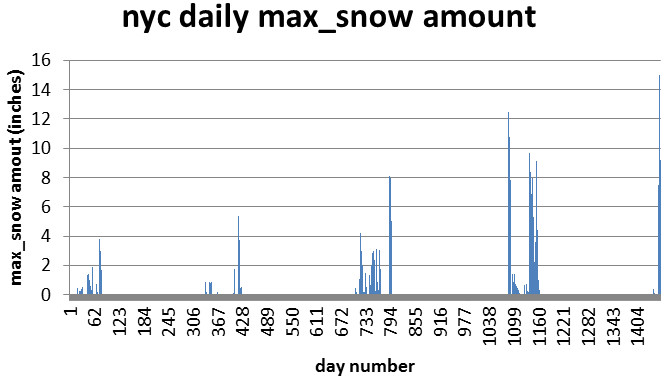
\includegraphics[width=3in,clip,trim=0 0.78in 0 0.5in]{plots/nyc_daily_maxsnow.png} \\
%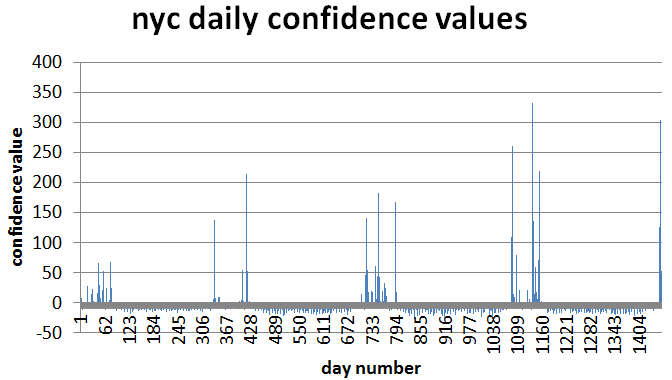
\includegraphics[width=3in,clip,trim=0 0 0 0.5in]{plots/nyc_daily_confidence.png} \\
\hspace{0.05in}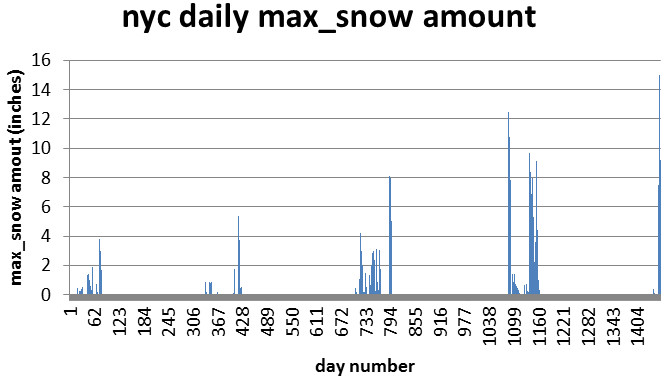
\includegraphics[width=2.66in,clip,trim=0 0.78in 0 0.5in]{plots/nyc_daily_maxsnow.png} \\
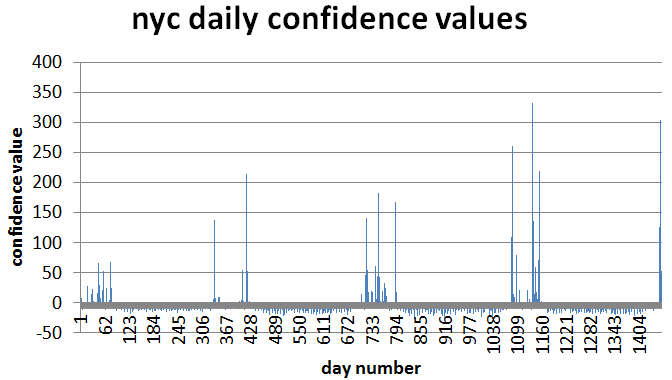
\includegraphics[width=2.7in,clip,trim=0 0 0 0.5in]{plots/nyc_daily_confidence.png} 
\end{tabular}
%\end{center}
\vspace{-12pt}
\caption{Time series of actual daily snow  (top) and score estimated from Flickr  (bottom) for New York City, 2007--2010.}
\label{fig:nyc_daily_conf_maxsnow}
\end{figure}
%
%
%
%% \begin{figure*}
%% \begin{center}
%% \begin{tabular}{cc}
%% 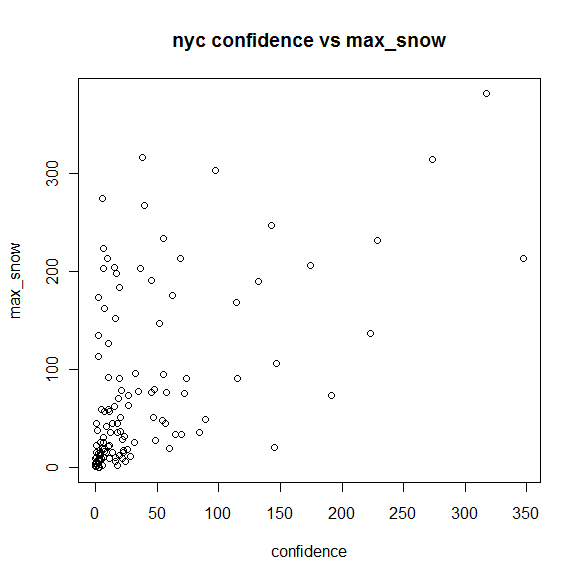
\includegraphics[width=0.5\textwidth]{plots/confidence_vs_maxsnow.png} &
%% 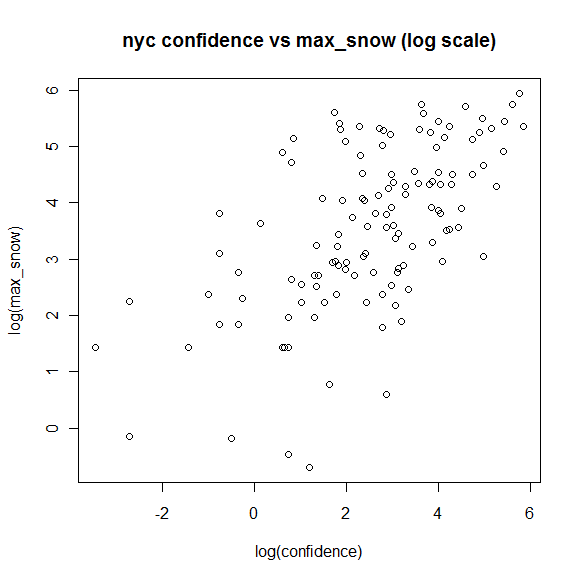
\includegraphics[width=0.5\textwidth]{plots/confidence_vs_maxsnow_log.png} \\
%% (a) & (b) \\
%% \end{tabular}
%% \end{center}
%% \caption{Scatter plots for days where confidence and max\_snow are both greater than 0 for NYC.}
%% \label{fig:confidence_vs_maxsnow}
%% \end{figure*}
%
%here goes our regression method
Because snow cover is temporally correlated, we fit a multiple linear regression model in which 
the confidence scores of the last several days are incorporated. The prediction on day $t$ is then
given by,
%
\begin{equation*}
\begin{cases}
\sum_{i=0}^T \alpha_{i} \log(conf_{t-i})+\beta & \mbox{ if $conf_t \geq 1$ } \\
0 & \mbox { otherwise } \\
\end{cases}
\end{equation*}
%
%\begin{equation*}
%\max\left( 0, \sum_{i=0}^T \alpha_{i}*conf_{t-i}+\beta \right),
%\end{equation*}
where $conf_t$ represents the likelihood ratio from
equation~(\ref{eq:conf}) on day $t$, $T$ is the size of the temporal
window, and the $\alpha$ and $\beta$ parameters are learned from the
training data.  We found that increasing $T$
generally improves performance on the 4 cities, but that no additional
improvement occurred with $T > 3$. We can measure the error of our
predictions with the root-mean-squared error between the time
series of our predictions and the actual snow data
(following~\cite{jin10prediction}).
%As Table~\ref{tab:prediction_stats} shows, w
We achieve an RMS error of
between about 1 and 1.5 inches across the 4 cities; Philadelphia has
the largest error (1.44), followed by Boston (1.26), New York (1.15), and Chicago (1.06).
As an example, Figure~\ref{fig:prediction_vis} presents a visual comparison of the
prediction time series versus the actual snow time series for Chicago. 







%% Then we first view the problem as a binary prediction
%% problem. Days with $max\_snow$ > 0 are snow days and days with
%% $max\_snow$ = 0 are non-snow days while days with $\hat{max\_snow}$ >
%% 0 are predicted as snow and days with $\hat{max\_snow}$ = 0 are
%% predicted as non-snow. FPR and TPR are computed. For FP (predicted as
%% snow, but actually no snow) cases, we compute average
%% $\hat{max\_snow}$ which shows that the predictions are not much larger
%% than 0. FN (predicted as no snow, but actually has snow) cases'
%% average $max\_snow$ are much smaller than TP (predicted as snow,
%% actually has snow) cases' average $max\_snow$ suggests that when the
%% negative (non-snow) predictions are wrong, the actual $max\_snow$
%% values are usually small which might result in few users tagging
%% snow. Then we come to snow range (multi-label) predictions.  We define
%% range\_off value to be:

An alternative way of evaluating the snow quantity estimates is to view
it as a multi-way classification task. 
We follow an existing snowfall impact scale~\cite{squires5} and
quantize daily snow quantity into 7 buckets: no snow, 0-1 inches, 1-4
inches, 4-10 inches, 10-20 inches, 20-30 inches, or more than 30
inches.  We then build a classifier to predict the snow
ranges for the four cities using the numbers of snow and non-snow users. We include
the numbers of users from the previous three days as extra
features. We use a Naive Bayesian classifier~\cite{john1995estimating}, which performed best on this task.
These multi-way classification results are  better than a majority class baseline, with 7-way correct classification rates
at 87.5\% for Philadelphia, 87.9\% for New York, 84.0\% for Boston, and 83.7\% for Chicago (versus baselines of 80.5\%, 85.1\%, 75.6\%, and 72.9\%, respectively).


%report the results from linear regression as well as the various statistics used in the table.

%% We define range\_off value to be:
%% \begin{equation*}
%% range\_off=|\hat{range\_num} - range\_num|
%% \end{equation*}
%% where $range\_num$ and $\hat{range\_num}$ are actual and predicted range numbers respectively.
%% Then we define n\_range\_off to be the total number of days with range\_off=n. The overall snow range accuracy will be 0\_range\_off/days\_in\_test.
%% The baseline method predicts all the days to be in range 0 which is the majority in the training set. All regression prediction results have better
%% snow range accuracy than the baseline results by margins from 3.9\% to 10.8\%.
%% For TP cases defined above in the binary prediction point of view for the regression model, we also calculate a loose snow range accuracy which is
%% (0\_range\_off+1\_range\_off)/TP. It shows that for TP cases (correct snow presence predictions), snow range accuracy is about 50\% and loose snow range accuracy is above 90\%
%% when $n$=3.



%I have not seen all the statistics, but I will write this conclusion for now.



%% \begin{table} 
%%  \caption {\textbf{Max\_snow ranges and corresponding range numbers}}
%% \label{tab:snow_ranges} 
%% \begin{center}
%% {\small{
%% \begin{tabular} {@{}|c@{}|c@{}|c@{}|c@{}|c@{}|c@{}|c@{}|c@{}|c@{}|} %{| \spa  r \spa | *{4}{\spa l \spa|}}   %{@{}c@{}c@{}c@{}c@{}c@{}}
%% \hline 
%%    %&   &  \textbf{\#}     %\tabularnewline
%% \textbf{range (inches)} &\textbf{0}  &\textbf{(0,1)} &\textbf{[1,4)}&\textbf{[4,10)} &\textbf{[10,20)}&\textbf{[20,30)}&\textbf{[30,$\infty$)}  \tabularnewline
%% \hline 
%% \textbf{range number} &\textbf{0} &\textbf{1} &\textbf{2} &\textbf{3} &\textbf{4} &\textbf{5} &\textbf{6}  \tabularnewline
%% \hline 
%% \end{tabular}}}
%% \end{center}
%% \end{table}


%We need to point out that confidence values help the ML method.
% we pointed that out in binary prediction and table for cities shows that for binary classification
% and it was mentioned in the text.


%figure for prediction results
\begin{figure}
\begin{center}
\begin{tabular}{c}
%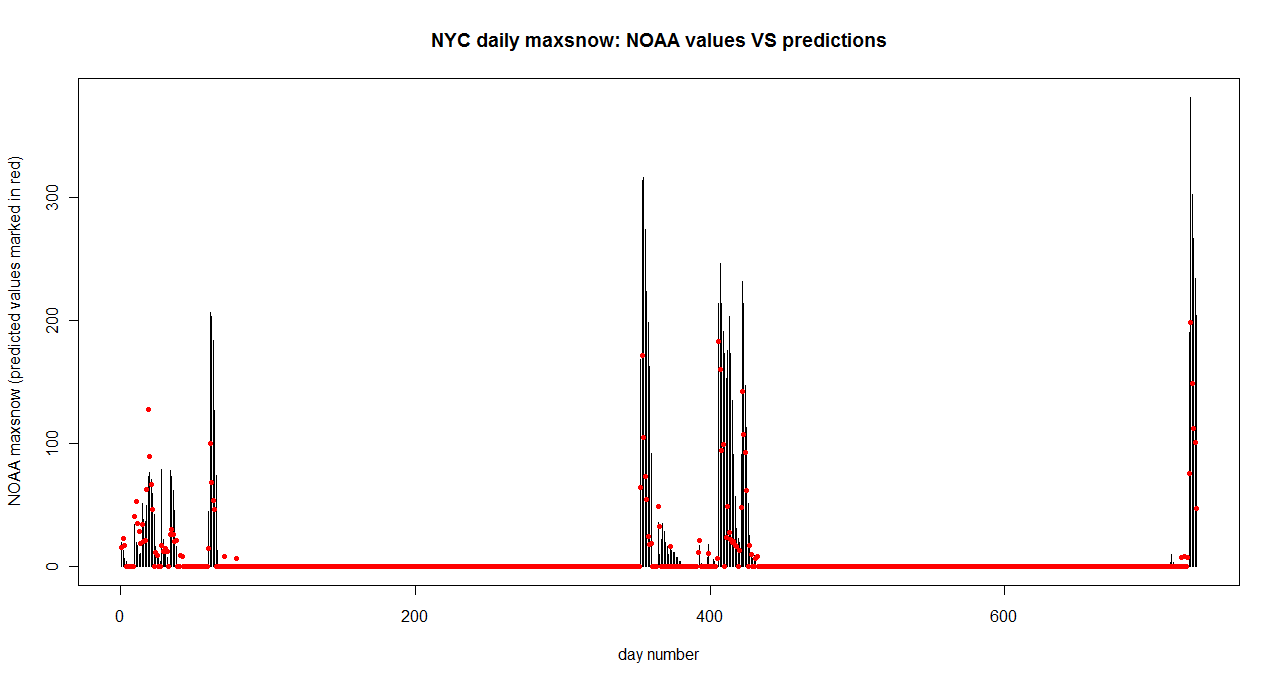
\includegraphics[width=0.5\textwidth]{plots/nyc_noaa_vs_prediction_prev_3.png} &
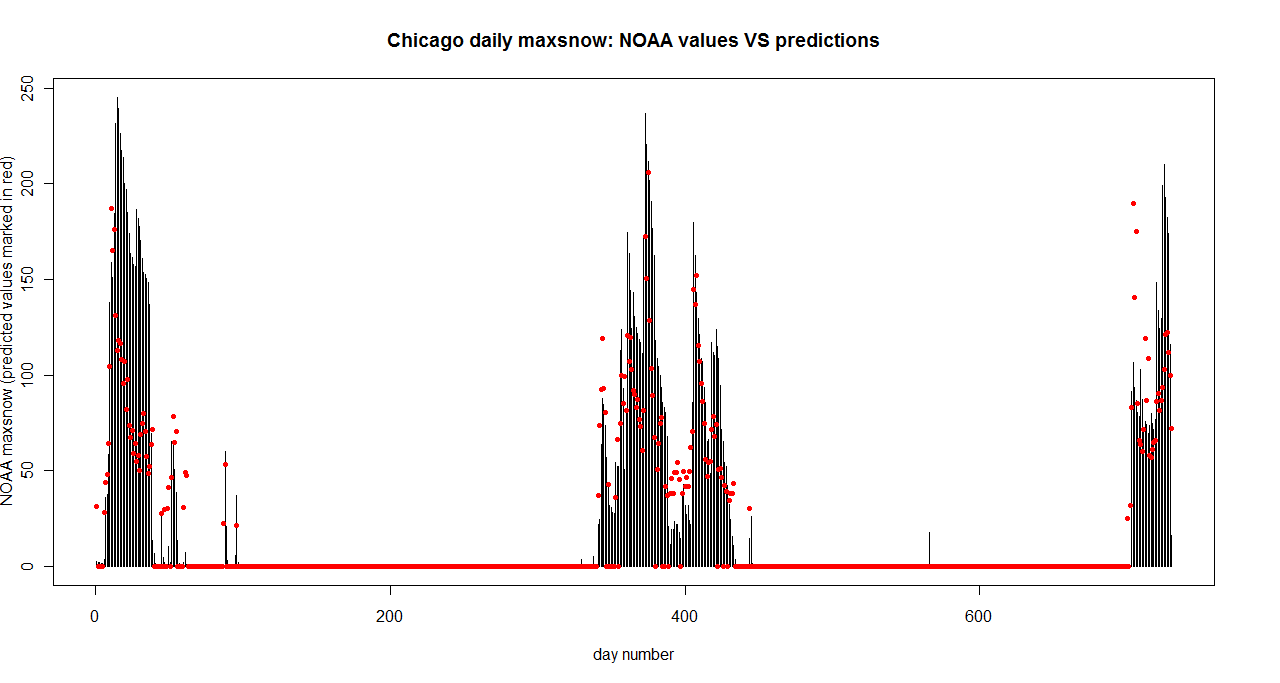
\includegraphics[width=0.5\textwidth,height=1.4in,clip,trim=0 0.5in 0in 0.6in]{plots/chicago_noaa_vs_prediction_prev_3.png} 
%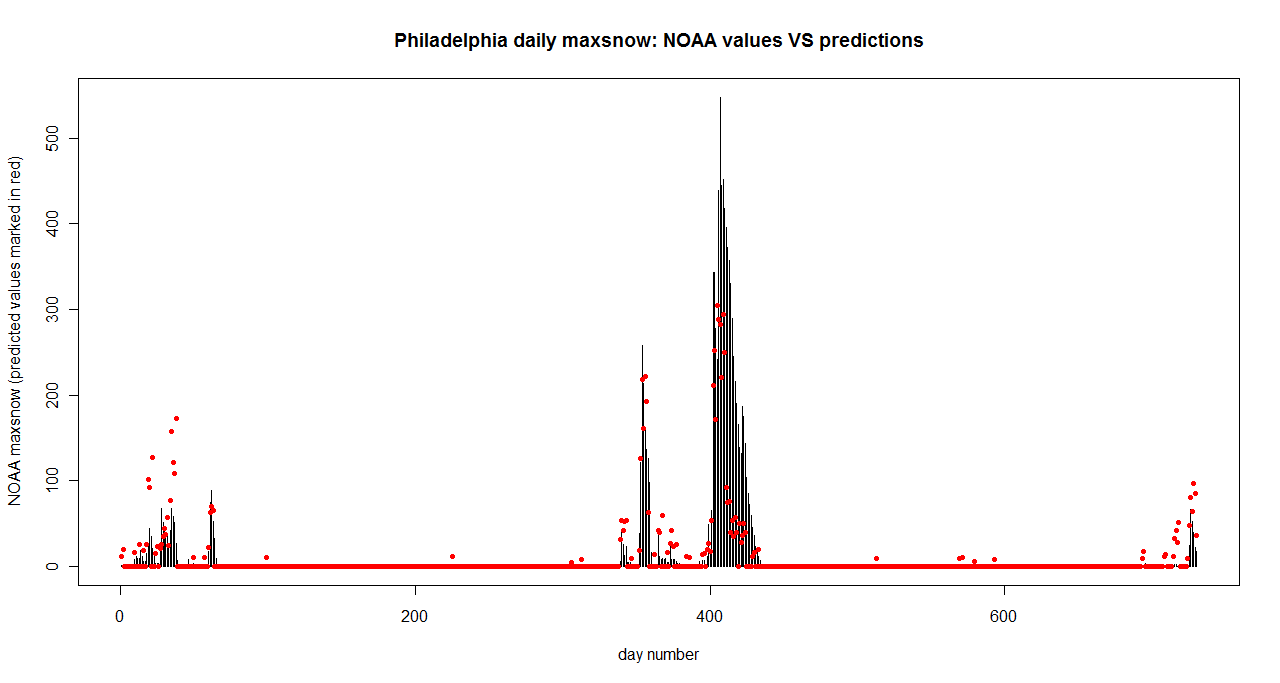
\includegraphics[width=0.3\textwidth]{plots/philly_noaa_vs_prediction_prev_3.png} \\
%(a) & (b) & (c)\\
\end{tabular}
\end{center}
\vspace{-24pt}
\caption{Comparing time series of actual daily snowfall (in mm) for Chicago with estimates using Flickr, for Jan 2009--Dec 2010 and $T=3$. Red dots show predictions, and vertical bars show actual values.}
\label{fig:prediction_vis}
\vspace{-12pt}
\end{figure}


%table for predictions statistics for confidence method

%% \begin{table} 
%%  \caption {\textbf{Max\_snow prediction statistics using linear regression method. (FP cases are the cases with $max\_snow$=0, predicted as snow;
%% TP are the cases with $max\_snow$>0, predicted as non-snow)}}
%% \label{tab:prediction_stats} 
%% \begin{center}
%% {\small{

%% \begin{tabular} {|p{2cm}|c|c|c|c|c|}
%% \hline 
%% \textbf{City} &\textbf{NYC}  &\textbf{NYC} &\textbf{Boston}&\textbf{Chicago} &\textbf{Phil.}   \\
%%  &\textbf{($T$=0)}  &\textbf{($T$=3)} &\textbf{($T$=3)}&\textbf{($T$=3)} &\textbf{($T$=3)}  \tabularnewline
%% \hline 
%% \textbf{RMS error} &{1.36} &{1.15} &{1.29} &{1.06} &{1.44}   \tabularnewline
%% \hline 
%% \textbf{Actual no snow days/actual snow days} &{621/109} &{621/109} &{552/178} &{532/198} &{588/142}   \tabularnewline
%% \hline 
%% \textbf{FP (predicted as snow, but no snow) Rate} &{1.1\%} &{1.1\%} &{3.3\%} &{0.2\%} &{2.9\%}   \tabularnewline
%% %&{7/621} &{7/621} &{18/552} &{1/532} &{17/588}   \tabularnewline
%% %\textbf{} 
%% \hline 
%% \textbf{TP (predicted as snow, actually has snow) Rate} &{69.7\%} &{69.7\%} &{79.2\%} &{79.8\%} &{64.8\%}   \tabularnewline
%% %{76/109} &{76/109} &{141/178} &{158/198} &{92/142}   \tabularnewline
%% \hline 
%% %\textbf{Precision} &\textbf{76/(76+7)} &\textbf{76/(76+7)} &\textbf{141/(141+18)} &\textbf{158/()} &\textbf{0.51}   \tabularnewline
%% %\hline 
%% \textbf{FP cases avg $\hat{max\_snow}$} &{0.75} &{0.33} &{1.08} &{0.88} &{0.51}   \tabularnewline
%% \hline 
%% \textbf{FN cases avg $max\_snow$} &{0.75} &{0.75} &{0.94} &{0.89} &{0.71}   \tabularnewline
%% \hline 
%% \textbf{TP cases avg $max\_snow$} &{4.11} &{4.11} &{4.06} &{3.96} &{3.98}   \tabularnewline
%% %\hline 
%% \hline 
%% \textbf{Snow range accuracy} &{89.0\%} &{88.9\%} &{82.5\%} &{83.7\%} &{84.5\%}   \tabularnewline
%% \hline 
%% %\textbf{Range 0+1 rate} &\textbf{0.9753425} &\textbf{0.9835616} &\textbf{0.9643836} &\textbf{0.9821918} &\textbf{0.9780822}   \tabularnewline
%% %\hline 
%% \textbf{Baseline snow range accuracy} &{85.1\%} &{85.1\%} &{75.6\%} &{72.9\%} &{80.5\%}   \tabularnewline
%% \hline 
%% %\textbf{Baseline Range 0+1 rate} &{0.9205479} &{0.9205479} &{0.830137} &{0.8027397} &{0.9164384}   \tabularnewline
%% %\hline 
%% \textbf{Snow range accuracy for TP} &{47.4\%} &{46.1\%} &{48.2\%} &{50.6\%} &{50.0\%}   \tabularnewline
%% \hline 
%% \textbf{Loose snow range accuracy for TP} &{84.2\%} &{92.1\%} &{97.9\%} &{100\%} &{93.5\%}   \tabularnewline
%% \hline 

%% \end{tabular}}}
%% \end{center}
%% \end{table}



%maybe we don't need to show the coefficients?
% mk, I agree with Haipeng , i commented  this part.
%%%%%%%%%%%%%%%%%%%%%%%%%%5
\begin{comment}
\textbf{$\beta$} &\textbf{0.69445} &\textbf{0.3386} &\textbf{1.1802} &\textbf{1.2691} &\textbf{0.6079}   \tabularnewline
\hline 
\textbf{$\alpha{}_{0}$} &\textbf{0.5213641} &\textbf{0.5061260} &\textbf{0.6014312} &\textbf{0.1615893} &\textbf{0.6219778}   \tabularnewline
\hline 
\textbf{$\alpha{}_{1}$} &\textbf{} &\textbf{0.2269894} &\textbf{0.5555687} &\textbf{0.5757585} &\textbf{0.6417626}   \tabularnewline
\hline 
\textbf{$\alpha{}_{2}$} &\textbf{} &\textbf{0.1390790} &\textbf{0.2696500} &\textbf{0.4327084} &\textbf{0.1076229}   \tabularnewline
\hline 
\textbf{$\alpha{}_{3}$} &\textbf{} &\textbf{0.1314299} &\textbf{0.5705873} &\textbf{0.2410475} &\textbf{1.0116489}   \tabularnewline
\hline 

\end{tabular}}}
\end{center}
\end{table}

\end{comment}
%%%%%%%%%%%%%%%%%%%%%%%%%






%%%%%%%%%%%%%%%%%%%%%%%%%%%%%%%mk   multi-class classification table (Snow range accuracy for zero_range and 1_range off


%% \begin{table} 
%%  \caption {\textbf{Snow range prediction statistics using Naive Bayesian classifier.}}

%% \label{tab:classifier_snow_range} 
%% \begin{center}
%% {\small{
%% \begin{tabular} {| p{2cm} | p{1cm} | p{1cm} | p{1cm} | c@{} |}
%% %\begin{tabular} {@{}|c@{}|c@{}|c@{}|c@{}|c@{}|c@{}|} %{| \spa  r \spa | *{4}{\spa l \spa|}}  
%% \hline 
%%  %&   &  \textbf{\#}     %\tabularnewline
%% \textbf {City} & \textbf{NYC} & \textbf{Boston}  &  \textbf{Chicago} &  \textbf{Philadelphia}   \tabularnewline
%% \hline
%% %\textbf {FP Rate} & (9/621) 1.4\%& (24/552) 4.3\%& (6/532) 1.1\%&(11/588) 1.8\%   \\   % \tabularnewline
%% \textbf {FP Rate} &  1.4\%&  4.3\%&  1.1\%& 1.8\%   \\   % \tabularnewline
%% \hline
%% \textbf {TP Rate} & 75.2\% &  93.8\%   &  93.4\%  &  78.2\%   \\   % \tabularnewline
%% \hline
%% \textbf {Snow range accuracy} &87.9\% & 84.0\%  & 83.7\%  & 87.5\%  \\   % \tabularnewline
%% \hline
%% \textbf {Snow range accuracy for TP} &36.6 \% & 50.9\% & 46.5\% & 55.9\%    \\   % \tabularnewline
%% \hline 
%% \textbf {Loose snow range accuracy for TP} & 87.8\% & 94.0\%& 94.1\% & 82.9\%   \\     %  \tabularnewline
%% \hline 

%% \end{tabular}}}
%% \end{center}
%% \end{table}



%\input{learningnoaa.tex}


\subsection{Continental-scale snow prediction}
Predicting snow  for individual cities is of limited practical use
because accurate meteorological data already exists for these highly
populated areas. In this section we ask whether phenomena can be
monitored at a continental scale, a task for which existing data
sources are less complete and accurate.  We use the photo data and
ground truth described in Section~\ref{sec:results}, although for the
experiments presented in this paper we restrict our dataset to North
America (which we defined to be a rectangular region spanning from 10
degrees north, -130 degrees west to 70 degrees north, -50 degrees
west). (We did this because Flickr is a dominant photo-sharing site in
North America, while other regions have other popular
sites --- e.g. Fotolog in Latin America and Renren in China.)  

The spatial resolution of the NASA satellite ground truth datasets is 0.05 degrees
latitude by 0.05 degrees longitude, or about $5 \times 5 km^2$ at the
equator.  (Note that the surface area of these bins is
non-uniform because lines of longitude get closer together near the
poles.)  However, because the number of photos uploaded to Flickr on
any particular day and at any given spatial location is relatively
low, and because of imprecision in Flickr geo-tags, we produce
estimates at a coarser resolution of 1 degree square, or roughly $100
\times 100 km^2$. To make the NASA maps comparable, we downsample them
to this same resolution by averaging the high confidence observations within the coarser bin.
We then threshold the confidence and snow cover percentages to annotate
each bin with one of three ground truth labels: 
%
\begin{packed_itemize}
\item[---] Snow bin, if confidence is above 90 and coverage above 80,
\item[---] Non-snow bin, if confidence is above 90 and coverage is 0,
\item[---] Unknown bin, otherwise.
\end{packed_itemize}
%
%hz: maybe should put it together with the Flickr confidence for that day to compare.
%djc: I think this is good enough, especially given our space constraints
Our goal is to predict whether or not each geospatial bin had snowcover on each day,
given the photos from Flickr.

%% Figure~\ref{fig:snowroc} presents an ROC curve for the
%% snow cover classification task, where again the goal is to decide
%% whether there was snow cover in each geospatial bin on each day, given
%% only the dataset of geo-tagged, time-stamped Flickr photos. As shown
%% in the curve, the likelihood ratio gives the best results, with the
%% voting and percentage methods performing significantly worse. For
%% example, at a false positive rate of 2.5\%, the confidence ratio gives
%% a true positive rate of about 92\%, while voting gives 86\% and
%% percentage gives about 80\%.
%% % The baseline probability (of a naive
%% %classifier that simply classifies all bins as non-snow) gives a true
%% %positive rate of 97.24\%.

%%  \begin{figure}
%%  \begin{center}
%%  \begin{tabular}{cc}
%%  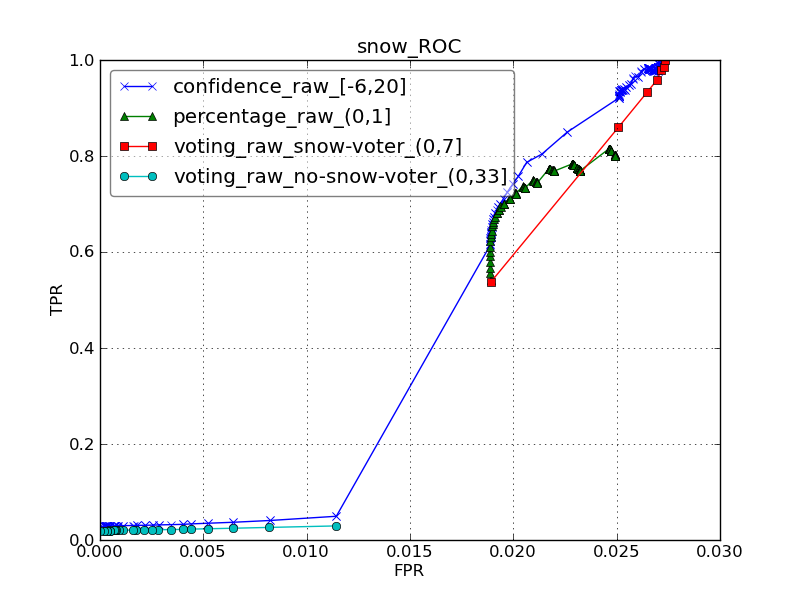
\includegraphics[width=0.4\textwidth,trim=1cm 1cm 1cm 1cm,clip]{plots/snow_roc.png}
%%  \end{tabular}
%%  \end{center}
%% \vspace{-12pt}
%%  \caption{ROC curve for the snow cover classification task.}
%%  \label{fig:snowroc}
%%  \end{figure}
%% %\begin{figure}
%% %\begin{center}
%% %\begin{tabular}{cc}
%% %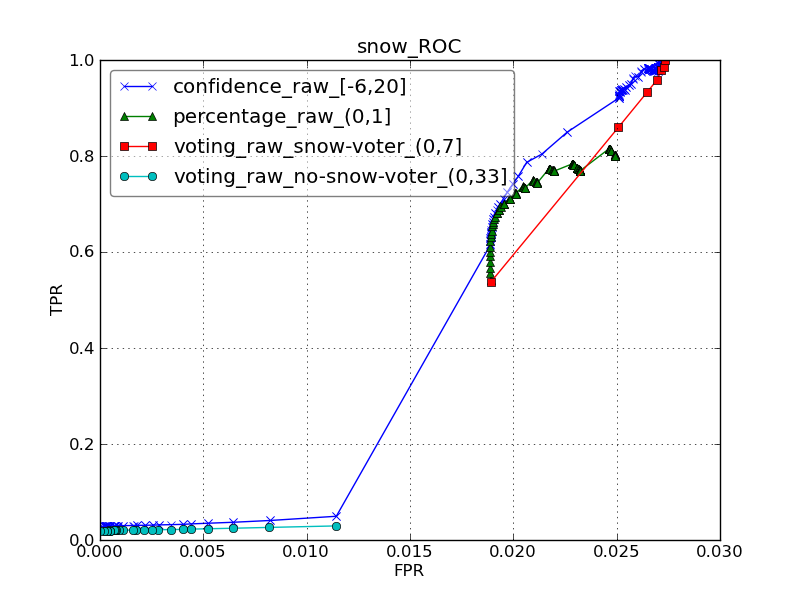
\includegraphics[width=0.4\textwidth]{plots/snow_roc.png}
%% %\end{tabular}
%% %\end{center}
%% %\vspace{-12pt}
%% %\caption{ROC curve for snow cover classification task}
%% %\label{fig:snowroc}
%% %\end{figure}


\begin{figure*}[ht!]
\begin{center}
\begin{tabular}{c|c|c}
  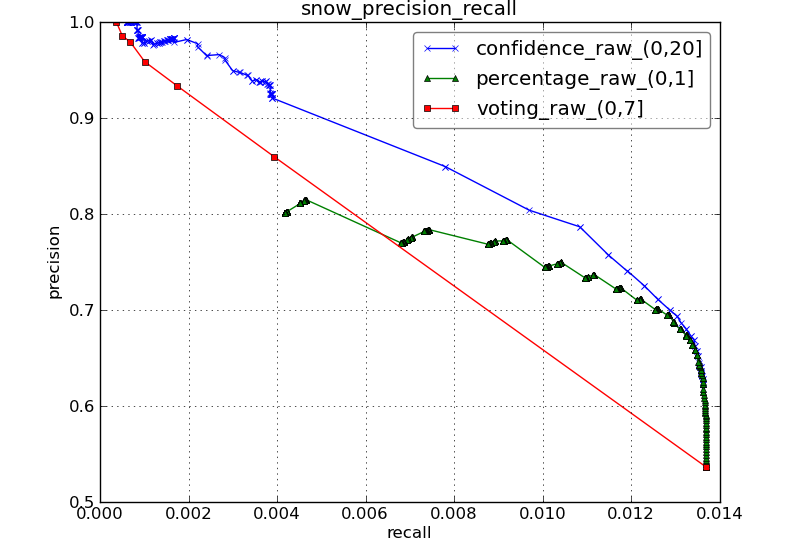
\includegraphics[width=0.32\textwidth,trim=1cm 0cm 1.5cm 0cm,clip]{plots/votingconfidencepercentage.png} & 
%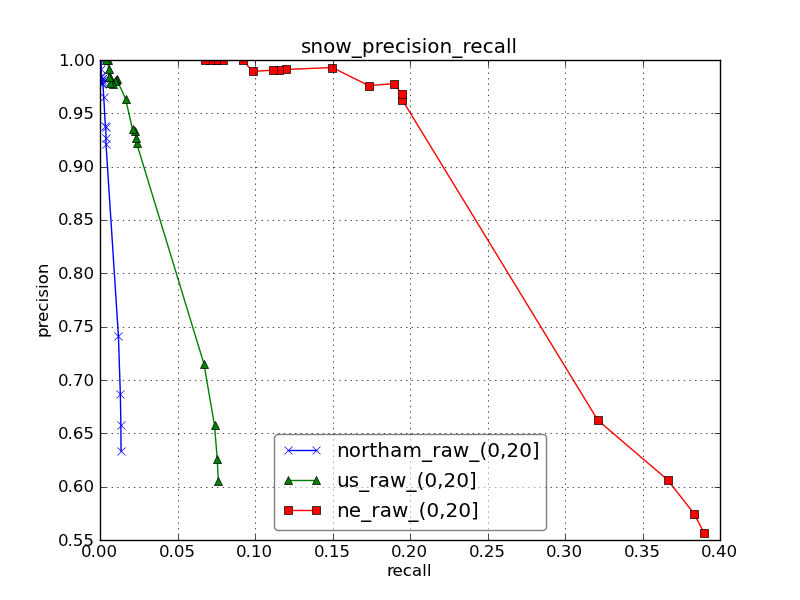
\includegraphics[width=0.32\textwidth]{plots/northamusne.png} & 
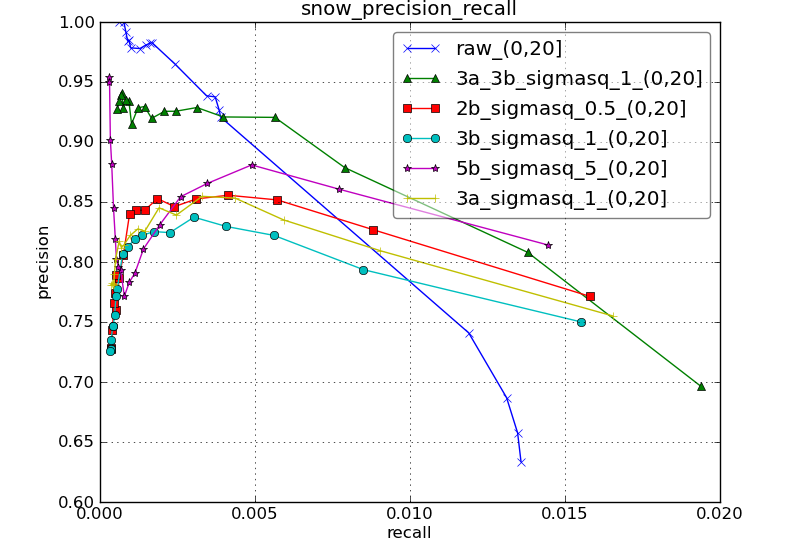
\includegraphics[width=0.32\textwidth,trim=1cm 0cm 1.5cm 0cm,clip]{plots/rawvsbest.png} &
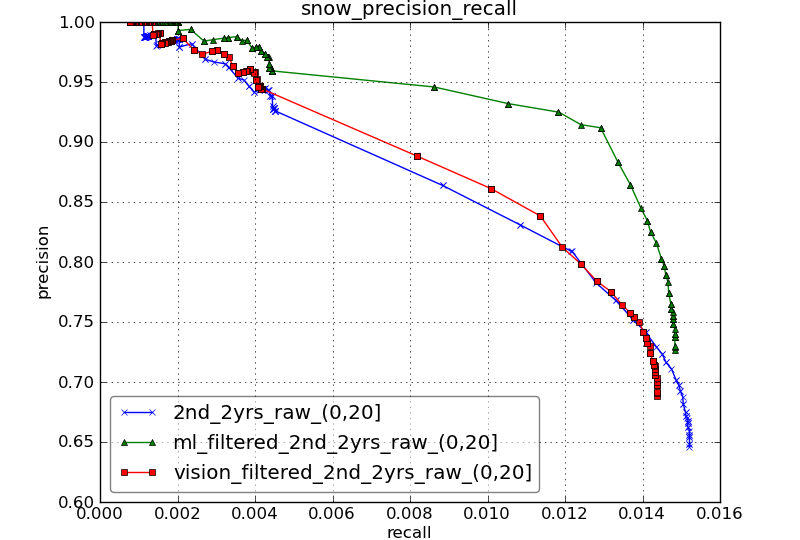
\includegraphics[width=0.32\textwidth,trim=1cm 0cm 1.5cm 0cm,clip]{plots/filtered_ml_vis_snow.png}\\
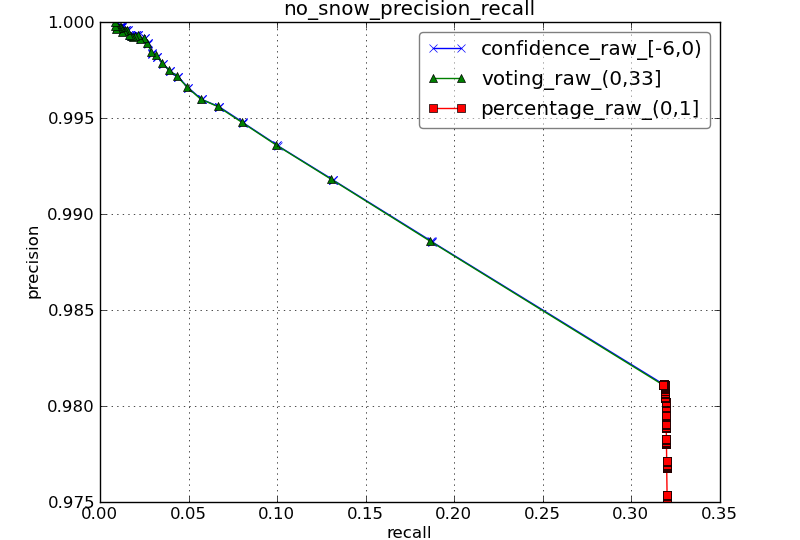
\includegraphics[width=0.32\textwidth,trim=0.7cm 0cm 1.5cm 0cm,clip]{plots/votingconfidencepercentagenosnow.png} & 
%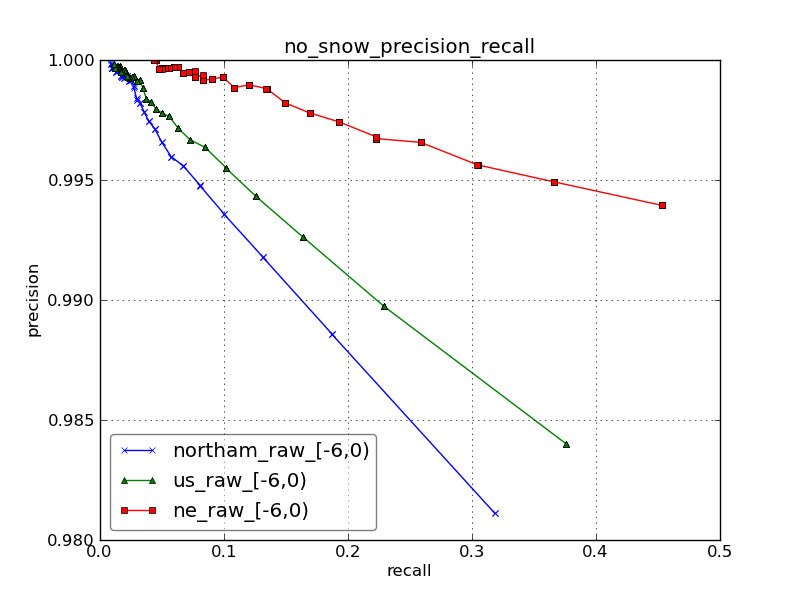
\includegraphics[width=0.32\textwidth]{plots/northamusnenosnow.png} & 
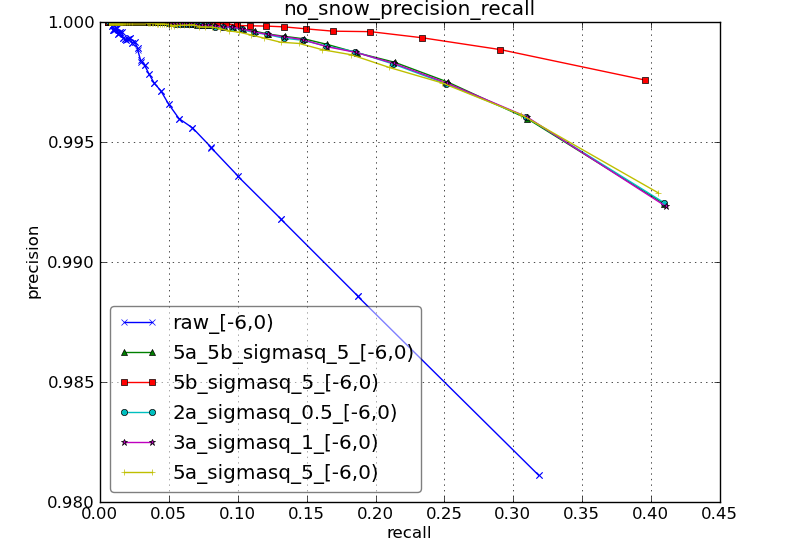
\includegraphics[width=0.32\textwidth,trim=0.7cm 0cm 1.5cm 0cm,clip]{plots/rawvsbestnosnow.png} &
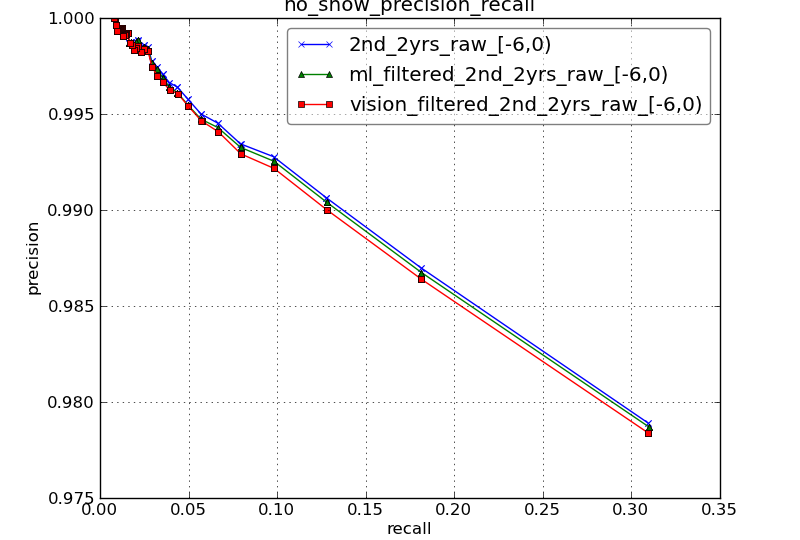
\includegraphics[width=0.32\textwidth,trim=0.7cm 0cm 1.5cm 0cm,clip]{plots/filtered_ml_vis_no_snow.png}\\
%(a) & (b) & (c) \\ 
%\\ \hline
%\\
%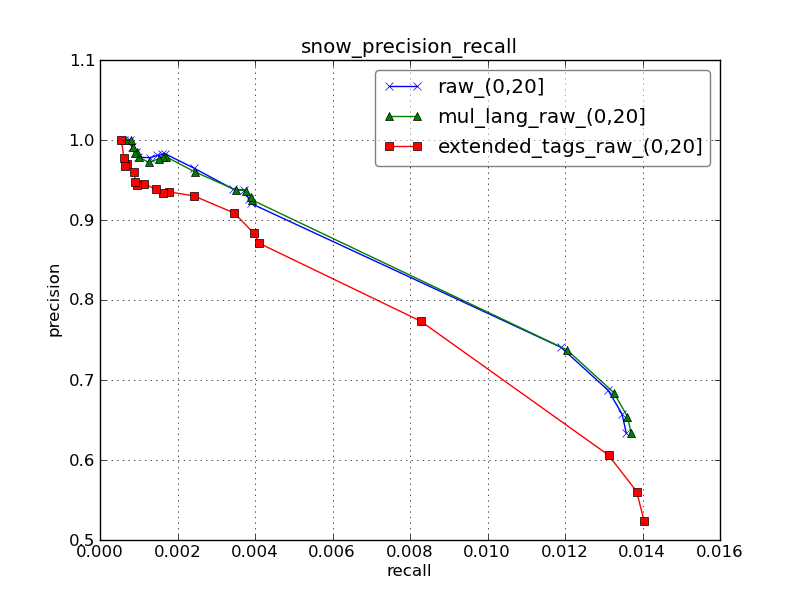
\includegraphics[width=0.32\textwidth]{plots/engmulextended.png} & 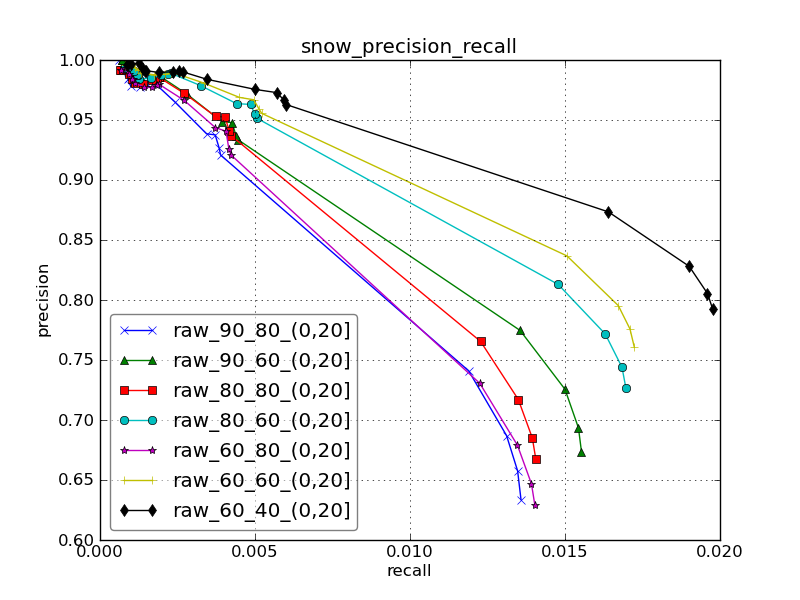
\includegraphics[width=0.32\textwidth]{plots/diffthresholds.png} & 
%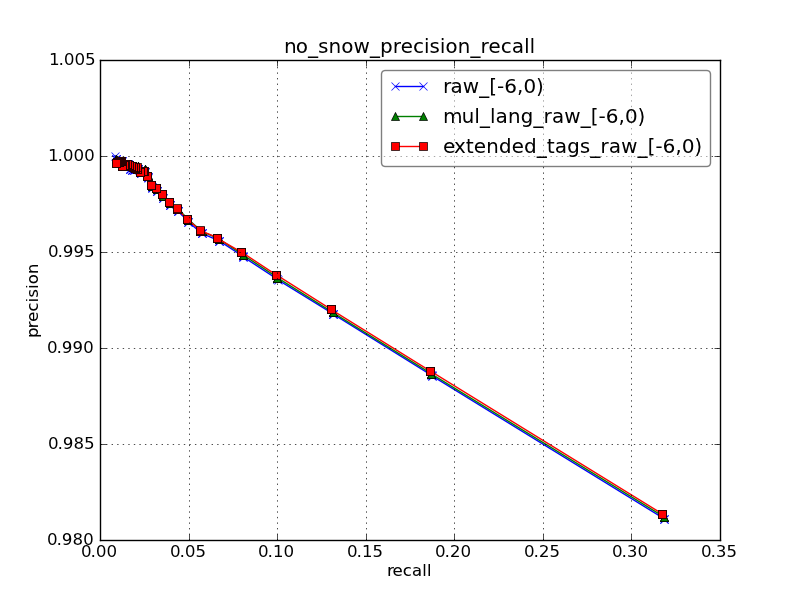
\includegraphics[width=0.32\textwidth]{plots/engmulextendednosnow.png} & 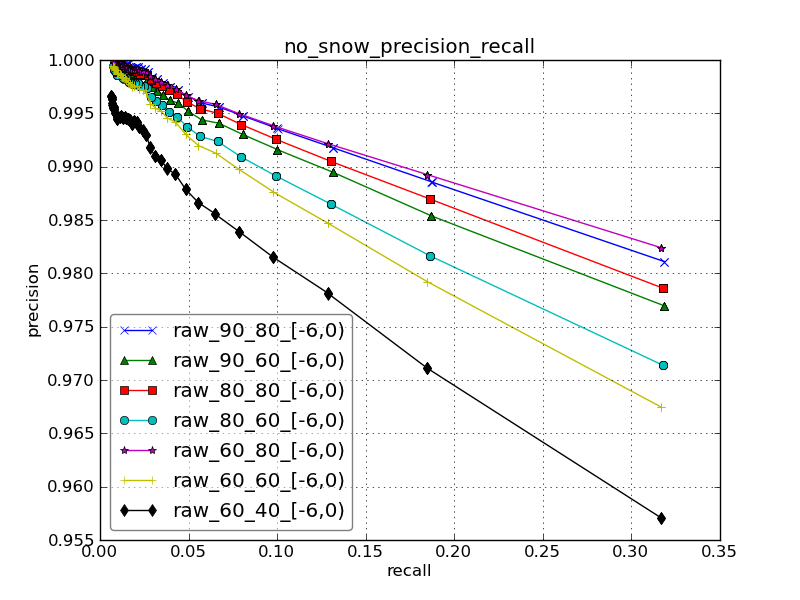
\includegraphics[width=0.32\textwidth]{plots/diffthresholdsnosnow.png} & 
(a) & (b) & (c) \\ 
%(d) & (e) & (f)\\
\end{tabular}
\end{center}
\vspace{-20pt}
\caption{Precision and recall curves for retrieving snow (top) and non-snow (bottom) instances, where an instance is a single geo-spatial bin on a single day, using different techniques: 
\textit{(a)} comparing the voting, percentage, and statistical confidence estimation techniques, 
%\textit{(b)} comparing performance on all of North America with just the continental U.S. and just the Northeastern U.S., 
\textit{(b)} comparing different temporal smoothing strategies, 
%\textit{(d)} comparing different sets of snow-related tags, 
%\textit{(e)} comparing different NASA ground truth thresholds, and 
\textit{(c)} using classifiers to reject falsely-tagged snow images using visual and textual features.}
\label{fig:votingconfidencepercentage}
\vspace{-12pt}
\end{figure*}

\xhdr{Retrieving snow or non-snow bins.}
In many real applications, ecologists would be satisfied in finding bins
for which the phenomenon is present, rather than actually classifying
all bins. It is thus useful to view this problem as a retrieval task,
in which the goal is to identify bins likely to contain the
phenomenon, or likely not to contain it. We thus turn to evaluating
the performance of our estimation techniques using precision-recall curves, where
%
\[
\begin{array}{cc}
\mbox{precision}=\frac{|R\cap G|}{|R|} \,\,\, &  \,\,\,
\mbox{recall}=\frac{|R\cap G|}{|G|}, \\
\end{array}
\]
%
where $R$ is the set of retrieved bins and $G$ is the set of correct
bins according to the ground truth.  Precision-recall curves are also
easier to interpret in situations where the classification baselines are so
high, as in our case.



%% \begin{figure}
%% \begin{center}
%% \begin{tabular}{cc}
%% 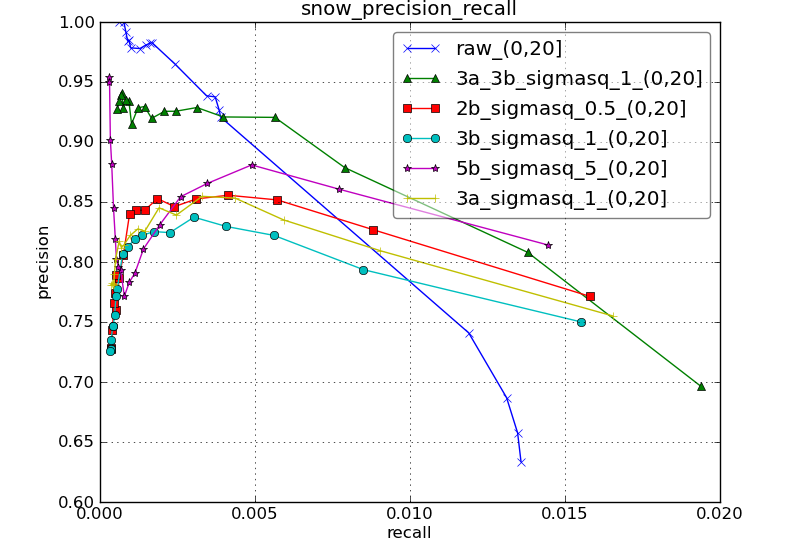
\includegraphics[width=0.5\textwidth]{plots/rawvsbest.png}
%% \end{tabular}
%% \end{center}
%% \caption{Precision and recall from different relatively good smoothing methods for snow predictions}
%% \label{fig:rawvsab}
%% \end{figure}

%% \begin{figure}
%% \begin{center}
%% \begin{tabular}{cc}
%% 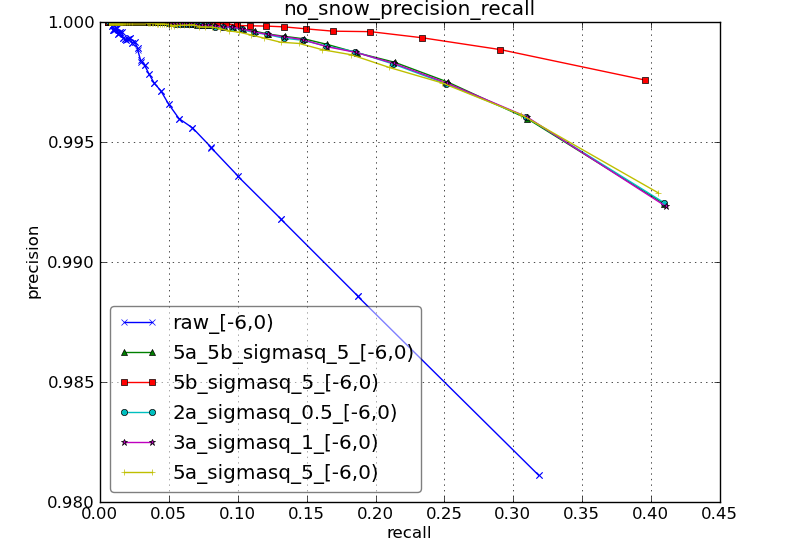
\includegraphics[width=0.5\textwidth]{plots/rawvsbestnosnow.png}
%% \end{tabular}
%% \end{center}
%% \caption{Precision and recall from different relatively good smoothing methods for no snow predictions}
%% \label{fig:rawvsabnosnow}
%% \end{figure}


%% \begin{figure}
%% \begin{center}
%% \begin{tabular}{cc}
%% 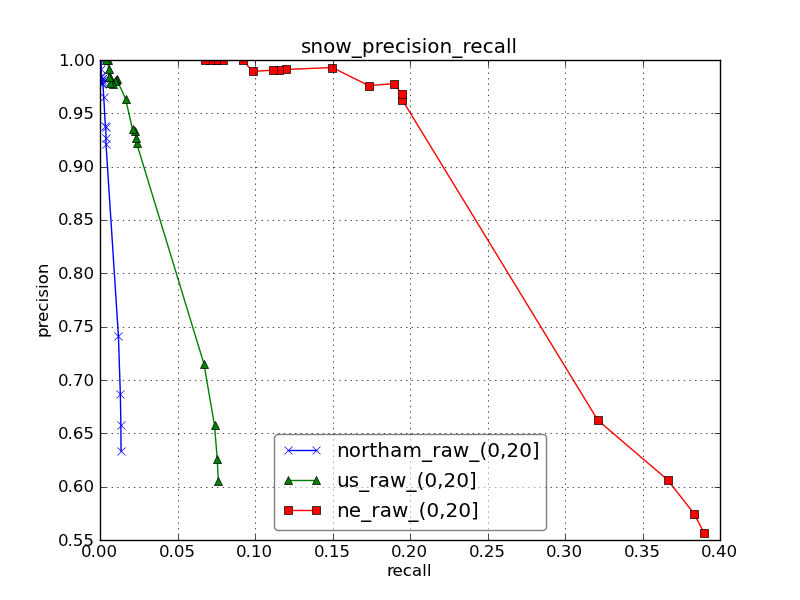
\includegraphics[width=0.5\textwidth]{plots/northamusne.png}
%% \end{tabular}
%% \end{center}
%% \caption{Precision and recall using Flickr data ranges of different density for snow predictions}
%% \label{fig:northamusne}
%% \end{figure}

%% \begin{figure}
%% \begin{center}
%% \begin{tabular}{cc}
%% 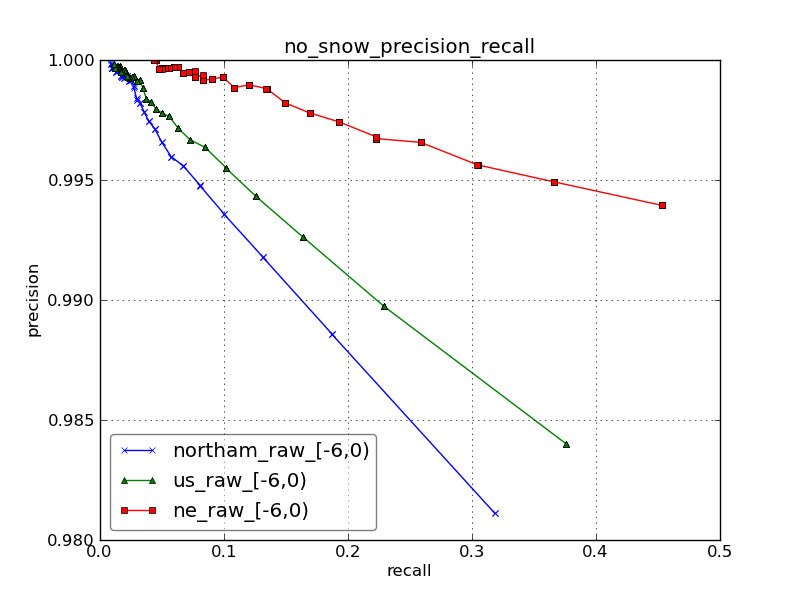
\includegraphics[width=0.5\textwidth]{plots/northamusnenosnow.png}
%% \end{tabular}
%% \end{center}
%% \caption{Precision and recall using Flickr data ranges of different density for no snow predictions}
%% \label{fig:northamusnenosnow}
%% \end{figure}


%\begin{figure}
%\begin{center}
%\begin{tabular}{cc}
%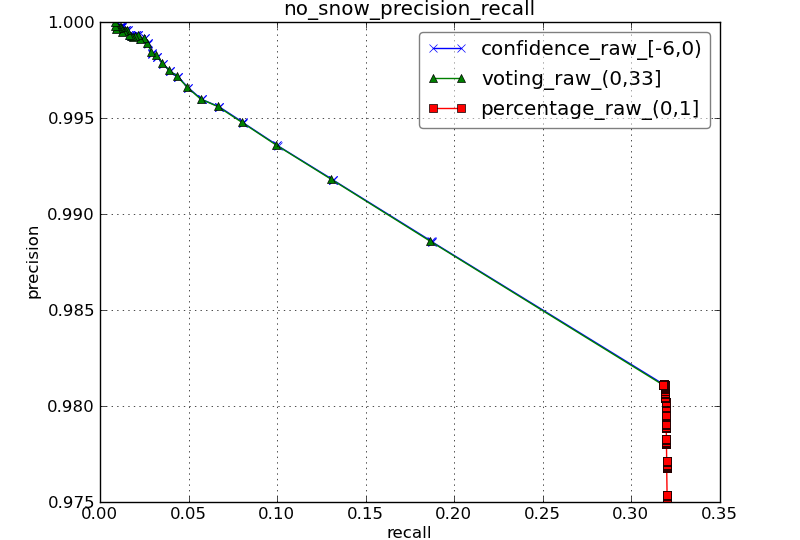
\includegraphics[width=0.5\textwidth]{plots/votingconfidencepercentagenosnow.png}
%\end{tabular}
%\end{center}
%\caption{Confidence, percentage and voting methods for no snow predictions}
%\label{fig:votingconfidencepercentagenosnow}
%\end{figure}


Figure~\ref{fig:votingconfidencepercentage}(a) shows precision-recall
curves for retrieving bins and days containing snow (top) and those
not containing snow (bottom).  In total, these curves involve
classifying about 7 million exemplars (each of which is a single geospatial
bin on a single day), of which 11.0\% have ground truth. 82.2\% of
the bins with ground truth are no-snow bins, while snow bins account
for 17.8\%.
We observe that the confidence method performs significantly better than the other two methods for retrieving snow bins, 
achieving about 98\% precision at 0.2\% recall, and about 80\% precision at 1\% recall. 
For retrieving non-snow bins the three techniques are almost the same, and all three perform better than the random baseline.

%\xhdr{Subregions with denser photo coverage.}
%\textbf{FIXME}  
While the precisions in these curves are high, the recall values are
alarming low. The main reason for this is that large areas of North
America, particularly most of Canada and Alaska, have sparse
populations resulting in a very limited number of photos uploaded in
these areas. We showed in the last section that accurate snow
estimates can be inferred for highly populated cities; the low recalls
here are because of low photographic density in much of the continent.
Restricting to specific subsets significantly increases the density of
observations: for example, the average number of photos per bin over
our four years of data is nearly ten times larger for the northeast US
compared to all of North America (70,398 vs 8,134).  The performance
is significantly better in these more densely populated areas; for
example, in the Northeast US the precision is 96.3\% at a recall of
19.5\% for snow retrieval, and 99.9\% precision at 9.1\% recall for
non-snow retrieval.  Moreover, recall would naturally improve as our
dataset grows; our sample of 150 million images is less than 3\% of
the photos on Flickr, and thus the recall would improve significantly
if we had access to the entire dataset.

\xhdr{Temporal smoothing.}  For many phenomena (including snow), the
existence of an event on one day is strongly correlated with its
existence on the next day. Thus one way of addressing the sparsity of
Flickr photos in some locations is to propagate evidence forward and
backward in time.  To do this, we apply a Gaussian filter on the Flickr
confidence values for each bin in an attempt to achieve better
recalls. We vary the degree of smoothing by using Gaussians with
different variance values. 
%For example, when the variance is 1, the
%effective temporal size of the filter is about 3 days. The confidence
%value of each day will be smoothed using the values from the range 3
%days before, 3 day after and itself.  
We tried smoothing with many
different parameters, including smoothing both forward and backwards
in time, or in only one direction.
Figure~\ref{fig:votingconfidencepercentage}(b) shows curves for
several of the best combinations that we found, including the raw
confidence score (blue X's), 3 days before and after with variance 1.0
%%hp cr: replaced sigma with variance.
(brown triangles), 2 days before with variance 0.5 (red squares), 3 days
before with variance 1.0 (blue circles), 5 days before with variance 5.0
(purple stars), and 3 days after with variance 1.0 (yellow +'s). We find
that temporal smoothing three days before and after with variance 1.0
%%(brown triangles), 2 days before with sigma 0.5 (red squares), 3 days
%%before with sigma 1.0 (blue circles), 5 days before with sigma 5.0
%%(purple stars), and 3 days after with sigma 1.0 (yellow +'s). We find
%%that temporal smoothing three days before and after with sigma 1.0
significantly improves performance for both snow and non-snow
retrieval, increasing snow retrieval precision by about 7 percentage
points at 1\% recall.

%% \xhdr{Expanded tag sets.}  We also try to improve the precisions and
%% recalls by expanding the list of snow-related tags. One way is to include multiple
%% languages(Spanish, Chinese, German, etc.) for snow related tags and
%% the other way is to include all the tags starting with ``snow'' such
%% as ``snowman.'' Using these heuristics, the number of snow-related tags 
%% expands to a set of 5,950, compared with only 4 in the previous experiments.
%%  Figure~\ref{fig:votingconfidencepercentage}(d) 
%% suggests that these additional tags do not improve
%% the results very much, and in fact the precisions for snow prediction actually drop.

%% \begin{figure}
%% \begin{center}
%% \begin{tabular}{cc}
%% 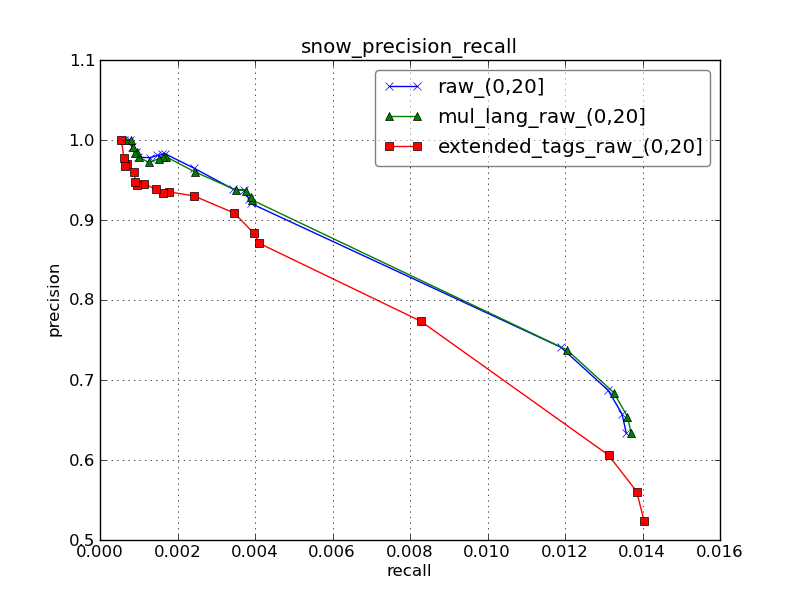
\includegraphics[width=0.5\textwidth]{plots/engmulextended.png}
%% \end{tabular}
%% \end{center}
%% \caption{Precision and recall using different snow tag lists for snow predictions}
%% \label{fig:engmulextended}
%% \end{figure}

%% \begin{figure}
%% \begin{center}
%% \begin{tabular}{cc}
%% 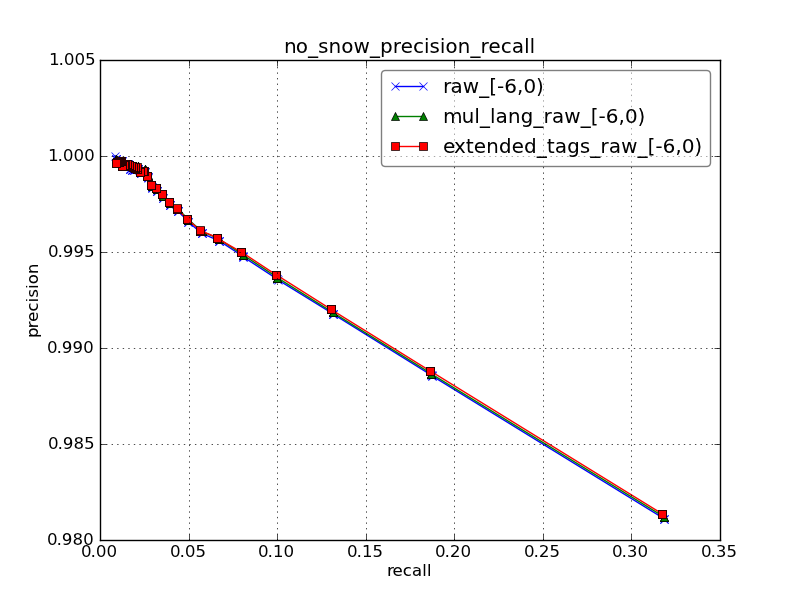
\includegraphics[width=0.5\textwidth]{plots/engmulextendednosnow.png}
%% \end{tabular}
%% \end{center}
%% \caption{Precision and recall using different snow tag lists for no snow predictions}
%% \label{fig:engmulextendednosnow}
%% \end{figure}

%% \xhdr{Alternative ground truth definitions.}  Finally, we compare
%% different definitions of snow and non-snow ground truth, by varying
%% the thresholds on the confidence and coverage in the NASA satellite
%% data. For each threshold combination, we fix the NASA no-snow
%% threshold to be 0 which means that only the bins without any snow will
%% be considered as no-snow bins. For all combinations, we adjust
%% different NASA confidence thresholds and NASA snow thresholds. When
%% these two thresholds are low, there will be more ground
%% truth. Figure~\ref{fig:votingconfidencepercentage}(e) shows that when NASA confidence
%% thresholds are fixed, lower NASA snow thresholds will result in higher
%% precisions and recalls but lower 
%% coverage thresholds will result in higher precisions and recalls. The curves
%% are ranked in reversed sequences in terms of overall precision and
%% recall in the two figures, which suggests a trade-off: the thresholds
%% that favor snow predictions harm no-snow predictions.

%% %when NASA snow thresholds are fixed, lower NASA confidence thresholds also improve precisions and recalls. 

%% \begin{figure}
%% \begin{center}
%% \begin{tabular}{cc}
%% 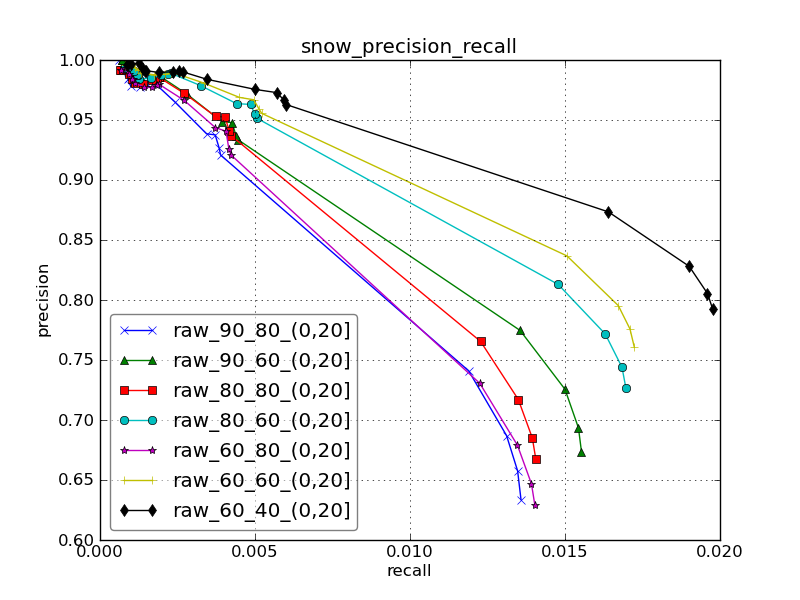
\includegraphics[width=0.5\textwidth]{plots/diffthresholds.png}
%% \end{tabular}
%% \end{center}
%% \caption{Precision and recall curves using ground truth from different thresholds for snow predictions}
%% \label{fig:diffthresholds}
%% \end{figure}

%% \begin{figure}
%% \begin{center}
%% \begin{tabular}{cc}
%% 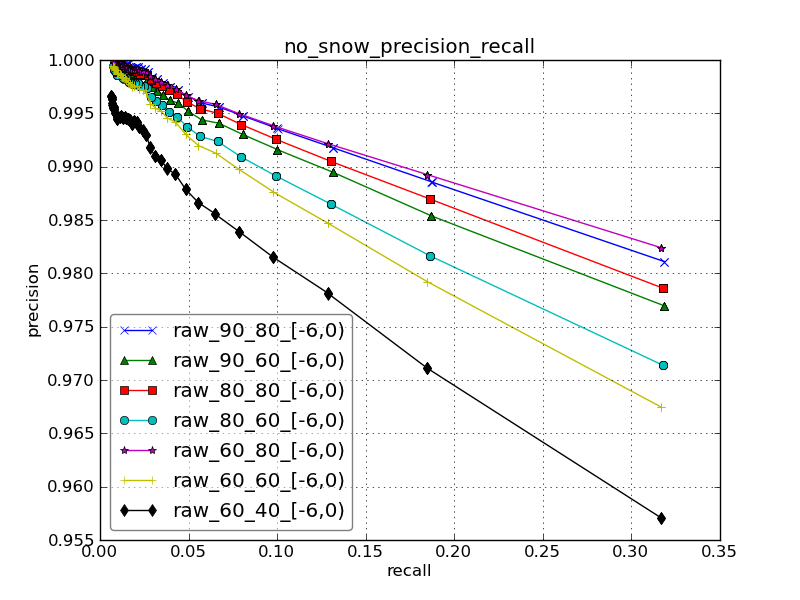
\includegraphics[width=0.5\textwidth]{plots/diffthresholdsnosnow.png}
%% \end{tabular}
%% \end{center}
%% \caption{Precision and recall curves using ground truth from different thresholds for no snow predictions}
%% \label{fig:diffthresholdsnosnow}
%% \end{figure}


\xhdr{Voting.}  Voting performs worse than the statistical confidence
given by the Bayesian likelihood ratio, but it is an interesting
technique to study in more detail because of its simplicity. Voting
simply counts the number of users who have annotated at least one
photo in a given bin and day with a snow-related tag.
Figure~\ref{fig:precvotes}
plots precision versus the number of votes for snow retrieval.  The
shape of these curve illustrates why crowd-sourced observations of the
world can be reliable, if enough people are involved: as the number of
votes for snow increases, it becomes progressively less likely that
these independent observations are coincidental, and more likely that
they are caused by the presence or absence of an actual phenomenon.
It is interesting to notice that when there are 7 or more snow voters,
snow prediction precision becomes 100\%, while the same is true for
non-snow prediction when the number of non-snow voters reaches 33
if there are no snow voters in the bin.

\begin{figure}
\begin{center}
\begin{tabular}{c}
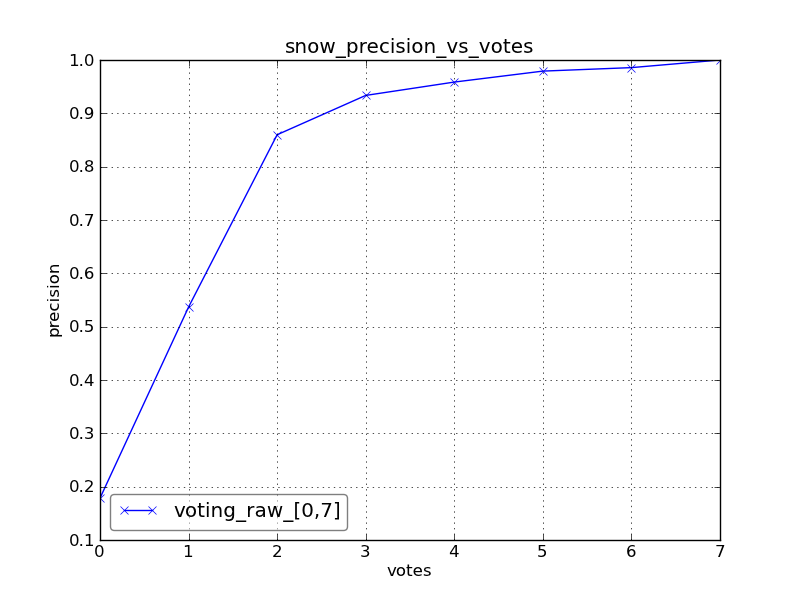
\includegraphics[width=0.3\textwidth,trim=1cm 0.5cm 1cm 1cm,clip]{plots/precvotes.png}
%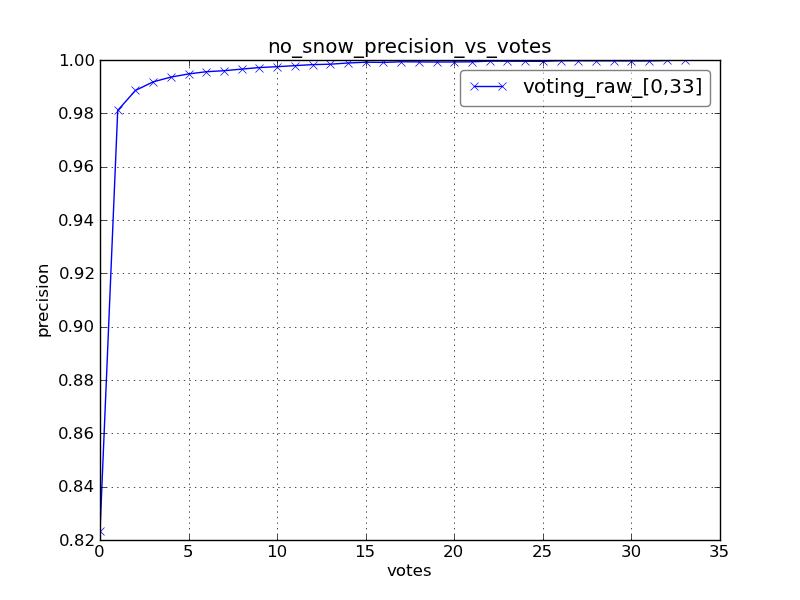
\includegraphics[width=0.3\textwidth,trim=1cm 1cm 1cm 1cm,clip]{plots/precvotesnosnow.png} \\
\end{tabular}
\end{center}
\vspace{-20pt}
\caption{Precision vs number of votes for snow predictions using the voting method.}
\label{fig:precvotes}
\end{figure}



%\label{sec:casestudy}

%For snow confidence value 5, we did a case study for wrong
%predictions. We checked the wrong predictions when using the raw data
%with confidence set to 5. The precision is 92.5\% and the recall is
%0.3\%. 6568 bins are predicted, 255 of which have ground truth and
%236 out of the 255 bins are correctly predicted. The 19 wrong cases
%have 46 photos and 38 of them are still available online. For each
%case, we checked the lat/lon of its first image to get the place from
%google maps. Then we used the place name and date to get the weather
%on that day. The tagmap-styled NASA data (error case marked in red on
%map) and raw NASA data is examined. For some cases, the error seems
%to be related to the resolution of bins, while for some cases, the
%error seems to be related to NASA satellite. We marked some
%interesting observations in red. See the case\_study.pdf
%(\url{http://www.cs.indiana.edu/~zhanhaip/flickr_vs_nasa/case_study.pdf})
%file.

%(405+180)+152+737+279+21
%Apr8_2011\wrong_case_snow_confidence_5
%Jul22_2011\download_img

\xhdr{Case study of false positives.}
To understand the failure modes of estimating attributes about the
world from Flickr photos, we performed a case study of false positives
--- bins and days in which our Flickr mining predicted the presence of
snow, but the NASA ground truth indicated that there was no snow
cover.  In particular, we studied snow false positives at the
operating point at which the likelihood ratio method gives a precision
of 74.1\% and a recall of 1.2\% (i.e. when the threshold is 4). At
this operating point, 34,323 total predictions are made (each
corresponding to a single geospatial bin on a single day), 2,208 of
which have valid ground truth.  Of these 2,208
bins, 1,636 (74.1\%) are correctly classified, while the 572 false
positive bins have a total of 1,855 photos tagged with one of the snow
terms (despite the fact that they were taken at places and times in
which the NASA satellite did not record snow).  We manually examined
these 1,855 false positive photos and classified them into 5 different
classes according to their visual content, as shown in
Table~\ref{tab:case_study_class}. Nearly 60\% of these photos do
actually appear to contain some snow; of these, 33\% either show trace
amount of snow or snow in the distance (usually on a distant mountain
peak), and 8.6\% have man-made snow that would not show up on the NASA
maps (like in a zoo or ski slope), while only about 16\% include a
significant amount of natural snow. About 40\% of the photos tagged
with a snow-related term do not appear to contain any snow at all; these
are caused by mis-tagged images or snow-related tags that are used to
describe something else (like the interference on a TV screen).
Figure~\ref{fig:casestudysample} shows some sample false positives from each class. 
% examining the tags of the photos, we notice that the tag
% ``snowegret'' is related to ``no-snow'' photos while the tag
% ``mountains'' is related to ``distant-snow'' photos. Also, some of
% the the ``snow'' photos appear to have timestamps in the
% summertime. These signal inspires the idea to learn a classifier
% based on the metadata of the photos to pre-process the snow tagged
% photos such that the photos without snow in content can be rejected
% to improve the precision of the snow/no snow prediction methods.

%: 1.``a little snow or distant snow'' that contains photos with a little snow or snow in distance in them, 2.``man made snow'' that contains snow made by human such as ski snow, 3.``no snow'' that contains photos without snow in them, 4.``snow'' that contains photos with much snow in them and 5.``not sure'' that contains photos that do not belong to other classes. Class 1 contains 33.0\% of the photos, class 2 contains 8.6\%, class 3 contains 41.5\%, class 4 contains 15.7\% and class 5 contains 1.2\%.
%hz: need a table for the statistics

\begin{table}[t]
 \caption {\textbf{Taxonomy of manually-labeled false-positive photos (which have at least one snow-related tag despite being taken at a snowless time and place according to the ground truth).}}
\label{tab:case_study_class} 
\begin{center}
\small{
\begin{tabular}{|l|p{4cm}|r@{\,\,}l|}
\hline 
\textbf{Class} & \textbf{Description} & \multicolumn{2}{c|}{\textbf{\# of photos}} \tabularnewline
\hline 
\hline 
little or distant   & photos with trace amount of snow or snow in the distance  & 585 & (33.0\%)\tabularnewline
\hline 
man made  & photos with snow made by humans (e.g. at a ski slope) & 152  & (8.6\%)\tabularnewline
\hline 
no snow & photos without visible snow  & 737 & (41.5\%)\tabularnewline
\hline 
snow & photos with significant snow  & 279 & (15.7\%)\tabularnewline
\hline 
not sure & other photos & 21 & (1.2\%)\tabularnewline
\hline 
\end{tabular}
}

\end{center}
\end{table}

\begin{figure}[th!]
\begin{center}
\begin{tabular}{cc}
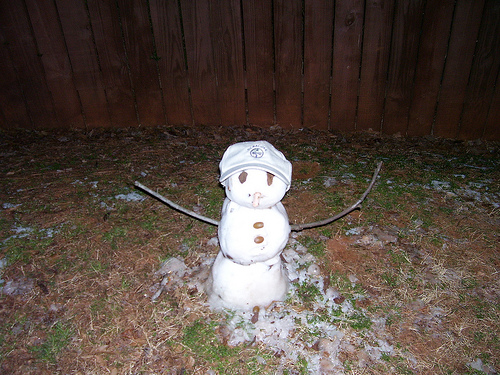
\includegraphics[width=0.16\textwidth]{plots/alittlesnow.jpg} &			%photo id 2210606613 tags atlanta snow toddler bowie snowtoddler
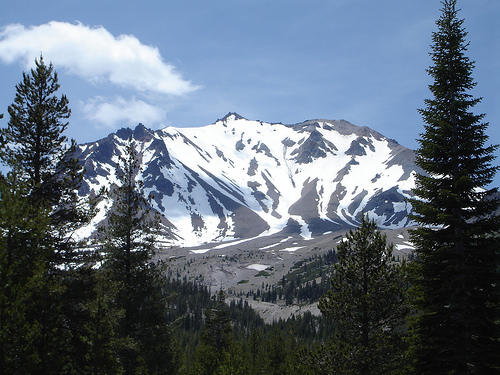
\includegraphics[width=0.16\textwidth]{plots/distantsnow.jpg} \\			%photo id 1963730656 tags blue park green forest trees white tree volcano snow mountain cloud
(a) & (b) \\ \\
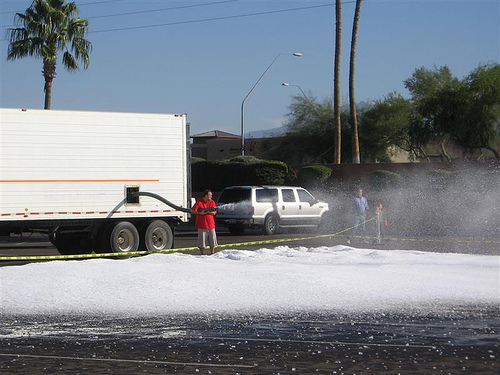
\includegraphics[width=0.16\textwidth]{plots/manmadesnow.jpg} &            %photo id 2041760519 tags tucson christmas snow arizona mall santa radio foothills kiim claus
\includegraphics[width=0.16\textwidth]{plots/nosnow.jpg} \\                     %photo id 2896829682 tags egret snowyegret water eau caribbean snowy blanc pond ciconiiformes antilles netherlandsantilles egretta caraïbes aigrette neigeuse thula etang whitte ardéidés egrettaneigeuse
(c) & (d) \\
\end{tabular}
\end{center}
\vspace{-15pt}
\caption{Sample photos that were not taken at a place and time with snow according to the ground truth, but that were uploaded with a snow-related tag:
  (a) photo with trace amounts of snow, (b) photo with distant snow, (c) photo with man made snow, and (d) photo with no snow (but with a ``snowy egret'').}
\label{fig:casestudysample}
\end{figure}

%hz, wrong cases: 1. wrong time stamps (wrong geo tags) 2. distant snow 3. some snow coverage, but entire bin is no-snow bin

For images that seem to contain natural snow, there are several possible explanations for why the ground
truth does not indicate snow cover at that time and place. One is that the
satellite passes over at an unknown time of day, so it is possible that snowfall occurred 
after the satellite's observation was taken.
Another cause are photos with incorrect time stamps or geo-locations; we
assume that such errors occur frequently, although it is hard to quantify the
frequency just by looking at the photos.
Other photos clearly contain snow, but the amount is so little 
that it might not be visible from the satellite (e.g.
Figure~\ref{fig:casestudysample}(a)), or the snow is so far in the distance
that it is in a different geospatial bin (e.g. Figure~\ref{fig:casestudysample}(b)).

%% \begin{figure} %[t]
%% \begin{center}
%% \begin{tabular}{cc}
%% \includegraphics[height=1in]{plots/distantphoto.jpg} &			
%% \includegraphics[height=1in]{plots/distantnasa.jpg} \\                    
%% (a) & (b) \\
%% \end{tabular}
%% \end{center}
%% \vspace{-15pt}
%% \caption{Example of a false positive caused by distant snow.
%% The photo in (a)
%% is located in the red box in the ground truth in (b), which is
%% Seattle. The white areas are water-covered, the purple areas are
%% snow-covered and the gray areas are snow-covered. There is no snow in
%% the red box and (a) may be capturing snow in
%% neighboring areas.
%% }
%% \label{fig:distant}
%% \end{figure}

There are some cases where the Flickr evidence for snow is overwhelming, but the NASA ground truth does not indicate snow.
This could be caused by the timing issue described above, or by 
satellite resolution and confidence issues. For example, on February 21, 2008, 5 Flickr users reported snowfall in New York.
This bin is marked as a
no-snow bin in the ground truth because the vast majority of it has zero snow coverage according to the satellite, but there is a 
small area within the bin that has low confidence (due to cloud cover) and probably corresponds to a snow squall.

%% \begin{figure}
%% \begin{center}
%% \begin{tabular}{cc}
%% \includegraphics[width=0.25\textwidth]{plots/nycnasa.jpg}
%% \end{tabular}
%% \end{center}
%% \caption{NASA data on 2008.2.21 for the New York City area. Black areas in the red box were covered by clouds.}
%% \label{fig:nyc}
%% \end{figure}
%% `
%According to the precision and recall curves, when the confidence threshold is higher, there will be less such prediction errors.

\xhdr{Machine learning for tag selection.}
%We are interested in solving some learning tasks. One task is to
%learn the snow tags using the human judged snow photos and non-snow
%photos together with their tags. %%Another task would be to determine
%whether snow-tagged photos contain snow visually using features such
%co-occurred tags, timestamps, geo stamps and visually features. Some
%tags combinations obviously reject snow-tagged photos, such as `snow,
%egret'.
Many of the above error modes can be addressed by training classifiers
on textual tag and visual images features.
%We now turn to an evaluation of how machine learning can be used to
%improve the quality of our estimates about the presence of ecological
%phenomena.  
As discussed in Section~\ref{sec:methods}, we are
interested in two learning paradigms: the first is to learn
combinations of tags that classify geospatial bins well according to
the NASA ground truth, while the second task is to reduce false
positives by rejecting photos that are tagged with a snow term but do
not actually contain snow.  
%All experiments here are done using 10
%fold cross-validation for evaluation, in which we split the training
%and test sets according to photographer (this prevents training data
%from leaking into the test data when the same user takes two very
%similar photos).

%\xhdr{Classifying bins.}
%
\begin{figure}
\begin{center}
\vspace{-12pt}
\begin{tabular}{c}
%\includegraphics[width=0.32\textwidth]{plots/DMNB_BINS_ALL_ROC.png} &
%\includegraphics[width=0.32\textwidth]{plots/DMNBtext_ReducedInfo_PrecRecall_1snow.png} &
%\includegraphics[width=0.32\textwidth]{plots/DMNBtext_ReducedInfo_PrecRecall_-1Nonsnow.png} \\
%\includegraphics[width=0.32\textwidth]{plots/LibLinear_All_info_TrainTest_Snow_1_curves_ROC.png} &
\includegraphics[width=0.32\textwidth]{plots/LibLinear_new_Bins4years2year2years_ROC_conf_IG_Tags_2.png} \\ 
%\includegraphics[width=0.32\textwidth]{plots/LibLinear_All_info_TrainTest_Snow_1_curves_PR_snow.png} &
%\includegraphics[width=0.32\textwidth]{plots/LibLinear_All_info_TrainTest_NonSnow_-1_curves.png} \\
% \includegraphics[width=0.25\textwidth]{plots/LibLinear_new_Bins4years2year2years_ROC_conf_IG_Tags.png} \\ (d) LibLinear_new_Bins4years2year2years_ROC_conf_IG_Tags.png may be used to show comparison between ML  classifier when tags , tags and information gain, tags+conf and conf method
% if we need to show comparison between ML and confidence method this figure could be used.
%%%% 
\end{tabular}
\end{center}
%<<<<<<< .mine
\vspace{-12pt}
\caption{ROC curves for classifying whether a geo-bin has snow on a given day, comparing the LibLinear classifier with various tag features to the confidence method using hand-selected tags.}
%=======
%\caption{Performance curves from LibLinear classifier, using the whole dataset with actual class label distribution when Information Gain and Confidence Methods are used to improve the classifier and when confidence methods used for prediction . }
%>>>>>>> .r1789
%(d) ROC curves when tags only,tags reduced by info-gain,confidence scores are used to build model }
\label{fig:dmnb-classifier}
\end{figure}
%
In the first task, we want to learn to classify whether a given bin
contains snow on a given day, based on a binary feature vector
encoding the set of tags used by all users in that bin on that
day.
% Our data set consists of 770,814 exemplars, each of which
%represents one bin in one day.  
%Of these samples only 208,626 contain
%images with tags.
We tried four different classifiers to address this problem: REPTree,
a fast decision tree learner which builds a decision tree using
information gain and variance and prunes it using reduced-error
pruning~\cite{hall2009weka}, Support Vector Machines
(SVMs)~\cite{CC01a}, Discriminative Multinomial Naive Bayes
(DMNB)~\cite{su2008discriminative} and LibLinear classifier with
L2-regularized logistic regression~\cite{Fan2008}.  To
reduce the large number of features (a total
of 404324 tags), we compute information gain and keep all
features (13442 tags) with information gain greater than
zero. 
%To avoid the unbalanced distribution of the samples of snow vs
%non-snow exemplars, we equalize the data by keeping all snow samples
%and randomly selecting the same number of non-snow
%samples. Table~\ref{tab:classifiers_bins} shows the classification
%results for the four classifiers; the best results are obtained by
%LibLinear while DMNB, SVMs and decision trees performed somewhat
%worse.
%
%% % mk, One should be used ROC for compare the 3 different classifiers  or PR curves .
%
%% Figure~\ref {fig:SnowBins_ROC_classifiers} shows the ROC curves when
%% DMNB,SVM,REPTree classifiers are used to classify snow bins vs
%% non-snow bins.  Figure~\ref{fig:NonSnowBins_classifiers} and ~\ref
%% {fig:SnowBins_classifiers} show the precision and recall in case of
%% classifying non-snow bins and snow bins for the three classifiers.
%
%
%% Also, we used DMNB to classify all the data without applying
%% equalization. DMNB achieved 97.77\% and baseline in this case is
%% 97.06( baseline is to predict the majority class non-snow in all
%% cases)\%.
%
%%%%%%%%%%%%%%%%%%%%%%The new table for 4 years data
Figure~\ref{fig:dmnb-classifier} presents ROC curves for this task, 
showing that the learned classifier outperforms the likelihood ratio from equation (\ref{eq:conf}), and that
feature selection with information gain and using the confidence ratio as an additional feature all improve performance.

%% \begin{table} 
%%  \caption {\textbf{ Comparison between LibLinear, DMNB, SVM and  REPTree classifiers in classifying presence of snow in bins.}}
%% \label{tab:classifiers_bins} 
%% \begin{center}
%% {\small{
%% \begin{tabular} {@{}|c@{}|c@{}|c@{}|c@{}|c@{}|c@{}|} %{| \spa  r \spa | *{4}{\spa l \spa|}}   %{@{}c@{}c@{}c@{}c@{}c@{}}
%% \hline 
%%    %&   &  \textbf{\#}     %\tabularnewline
%% \textbf{Classifier} & \textbf{Precision}  &  \textbf{Recall} & \textbf{F-Measure}&  \textbf{Accuracy}   \tabularnewline
%% \hline 
%% \textbf{LibLinear} & \textbf{0.816} &\textbf{0.815} & \textbf{ 0.815} & \textbf{0.815}   \tabularnewline
%% \hline 
%% \textbf{DMNB} & 0.827 &  0.812 &  0.809 & 0.812   \tabularnewline
%% \hline
%% \textbf{SVM} &  0.808 &  0.808 & 0.808 & 0.808  \tabularnewline
%% \hline 
%% \textbf{REPTree} & 0.766 &0.766   &  0.766    & 0.766\tabularnewline
%% \hline 
%% \end{tabular}}}
%% \end{center}
%% \end{table}



%%%%%%%%%%%%%%%%%%%%%%%%%%%old table
\begin {comment}
 Figure~\ref{fig:dmnb-classifier}(a) shows the ROC and precision-recall curves for DMNB.

\begin{table} 
 \caption {\textbf{ Comparison between  DMNB, SVM and  REPTree classifiers in classifying presence of snow in bins.}}
\label{tab:classifiers_bins} 
\begin{center}
{\small{
\begin{tabular} {@{}|c@{}|c@{}|c@{}|c@{}|c@{}|c@{}|} %{| \spa  r \spa | *{4}{\spa l \spa|}}   \hline 
\textbf{Classifier} & \textbf{Precision}  &  \textbf{Recall} & \textbf{F-Measure}&  \textbf{Accuracy}   \tabularnewline
\hline 
\textbf{DMNB} & \textbf{0.834} &\textbf{0.817} & \textbf{ 0.814} & \textbf{0.817}   \tabularnewline
\hline
\textbf{SVM} &  0.804 &  0.803 & 0.803 & 0.803  \tabularnewline
\hline 
\textbf{REPTree} & 0.768 &0.769   &  0.769    & 0.769\tabularnewline
\hline 
\end{tabular}}}
\end{center}
\end{table}
\end{comment}
%%%%%%%%%%%%%%%%%%%%%%%%%%%%%%%%%%%%%%%%%%%%%%%%%%%%%%%%%%%%%%%%%%%%%%%%%%%%%%%%%%%%%%%%%%%%%%%%

% mk, One should be used ROC for compare the 3 different classifiers  or PR curves .
 %%%%%%%%%%%%%%%Here are ROC curves
%% \begin{figure}
%% \begin{center}
%% \begin{tabular}{cc}
%% \includegraphics[width=0.5\textwidth]{plots/BINS_EQ_ROC_NASA.png}
%% \end{tabular}
%% \end{center}
%% \caption{ROC curves for using SVM, DMNB and REPTree classifiers}
%% \label{fig:SnowBins_ROC_classifiers}
%% \end{figure}



%%%%%%%%%%Here are PR curves%%%%%%%%%%%%%%%%%%%%%%%%%%%%%%%%%%%%%%%%%%%%%%%%%%%

%% \begin{figure}
%% \begin{center}
%% \begin{tabular}{cc}
%% \includegraphics[width=0.5\textwidth]{plots/Snow_Bins_NASA_EQ_Reduced.png}
%% \end{tabular}
%% \end{center}
%% \caption{Precision and recall using SVM, DMNB and REPTree for snow Bins}
%% \label{fig:SnowBins_classifiers}
%% \end{figure}


%% \begin{figure}
%% \begin{center}
%% \begin{tabular}{cc}
%% \includegraphics[width=0.5\textwidth]{plots/NonSnow_Bins_NASA_EQ_Reduced.png}
%% \end{tabular}
%% \end{center}
%% \caption{Precision and recall using SVM, DMNB and REPTree for non-snow Bins}
%% \label{fig:NonSnowBins_classifiers}
%% \end{figure}








%%%%%%%%%%%%%%%%%%%%%%%%%%%%%%%%%%%%%%%%%%%%%%%%%%%%%%%%%%%%%%%%%%

%\xhdr{Classifying photos} 
Next we try the second learning paradigm, in which our 
goal is to examine 
photos that have a snow-related tag, and use the other tags as well as visual features to decide
whether or not they actually contain snow. For example, the classifier
might learn that a photo with ``snowy'' should be discarded if it also
contains the tag ``egret,'' since that photo is likely of a bird and
not of actual snow.  
For training these classifiers, we had a human judge evaluate 1,855 images 
and to annotate them as to whether or not they actually contain evidence of snow.
%For this latter source of ground truth, we exclude the 15\% of photos actually containing snow from negative exemplars,
%and combine the 
%photos from ``a little snow or
%distant snow,'' ``man made snow'' and ``no snow'' into one category
%representing the negative class. Also,  we limit contribution of any one user by sampling 
%one image per day per bin per user. 

%%%%%%%%%%%%%%%%%%%%%%%%%%%%%%%%%%%%
% DTree
We used decision trees for this task because it is easy to understand
and interpret what features the classifier is using.  In initial
experimentation, we found that many of the most discriminative
features were place names, like ``sandiego'' or ``canada.'' These
geographic tags are understandably strongly correlated with snowfall,
but we would like our classifier to base its decisions on the content
of an image (because, for example, climate change might cause snowfall
in San Diego some day, and we would like our classifier to be able to
detect this).  To avoid selecting these tags, we first divide North
America into four regions (northeast, northwest, southeast, southwest)
and get the intersection of the sets of tags used in these four
regions.  We then use only this set of intersected tags
(``IntersTags'') for building the decision tree. Besides tags, we also
tried including the photo's timestamp month as an additional feature.

%% \begin{table}
%% \begin{center}
%% \small{
%%  \label{tab:classifier_Photos} 
%% \caption{\textbf{ Decision tree classification results using combinations of all tags and spatially intersected tags, with and without time (month) features, for NASA and human-judged ground truth.}}
%% \begin{tabular} {@{}|l@{}|c@{}|c@{}|c@{}|c@{}|} %{| \spa  r \spa | *{4}{\spa l \spa|}}   %{@{}c@{}c@{}c@{}c@{}c@{}}
%% %\begin{tabular} {|l|c|c|c|c|} %{| \spa  r \spa | *{4}{\spa l \spa|}}   %{@{}c@{}c@{}c@{}c@{}c@{}}
%% \hline 
%%    %%%&   &  \textbf{\#}     %\tabularnewline
%% \textbf{Features} & \textbf{Precision}  &  \textbf{Recall} & \textbf{F-Measure}&  \textbf{Accuracy}    \tabularnewline
%% \hline 
%% \textbf{AllTags} &0.903  &   0.908  &   0.893 & 0.908\tabularnewline
%% \hline 
%% \textbf{IntersTags} &0.88     & 0.893  &   0.873 &  0.893    \tabularnewline
%% \hline 
%% \textbf{AllTags+Time}  & \textbf {0.945}    &  \textbf{0.947}   &  \textbf{0.944} & \textbf{0.947}  \tabularnewline
%% \hline 
%% \textbf{IntersTags+Time} &0.94 &     0.942  &   0.938 & 0.942  \tabularnewline
%% \hline
%% %\textbf{AllTags, NASA GT} &  0.874   &  0.882   &  0.863 & 0.882 \tabularnewline
%% %\hline 
%% %\textbf{IntersTags, NASA GT}   &0.851    & 0.866   &  0.84  & 0.866 \tabularnewline
%% %\hline 
%% %\textbf{AllTags+Time NASA GT} &  \textbf {0.932}    & \textbf {0.934}  & \textbf { 0.93}  & \textbf {0.934} \tabularnewline
%% %\hline 
%% %\textbf{IntersTags+Time, NASA GT}  &0.926    & 0.927    &  0.922 & 0.927    \tabularnewline
%% %\hline
%% \end{tabular}
%% }
%% \end{center}
%% \end{table}


%%%%%%%%%%%%%%%%%%%%%%%%%%%%%%%%%%%%%%%%%%%%%%%%%%%%%%%%%%%%%%%%%%%%%ROC figures
\begin{figure}
\begin{center}
\vspace{-12pt}
\begin{tabular}{c}
%\includegraphics[width=0.33\textwidth]{plots/PhotosLimitUser_ROC_NASA.png} \\
\includegraphics[width=0.33\textwidth]{plots/PhotosLimitUser_ROC_Human.png}
\end{tabular}
\end{center}
\vspace{-20pt}
\caption{ROC curve for classifying whether photos contain snow, using decision trees with various features: AllTags includes all tags, IntersTags excludes tags 
corresponding to specific geographic areas, and AllTags+Time and IntersTags+Time include the month of the year as an additional feature.} 
\label{fig:PhotosLimitUser_ROC_NASA}
\vspace{-12pt}
\end{figure}

%%%%%%%%%%%%%%%%%%%%%%%%%%%%%%%%%%%%%%%%%%%%%%%%%%%%%%%%%%%%%%%%%%%%%%

ROC curves are presented in 
Figure~\ref{fig:PhotosLimitUser_ROC_NASA}. We
see that the time feature helps in improve the results, as does
using all tags instead of just the spatially-intersected ones.  The
baseline (majority class) is
86.3\%.
It is interesting to examine the top few levels of the trained decision tree,
to get a sense for which tags are most discriminative. The top decision
node is ``summer:'' if this tag is present, then the photo is classified as not snow.
If summer is not present, then the next few layers look at tags like ``mountain,'' ``clouds,'' ``ski,'' ``geese,'' and ``egret.''


%%%%%%%%%%%%%%DTree Figure 
%% \begin{figure}
%% \begin{center}
%% \begin{tabular}{cc}
%% \includegraphics[width=0.5\textwidth]{figs/Top_two_level_DTree.png}
%% \end{tabular}
%% \end{center}
%% \caption{Top 3 levels of REPTree when InterSet Tags are used and ground truth is human judged , 1 is now and -1 is non snow 
%% Tree visualized using weka ~\cite{hall2009weka} }
%% \label{fig:Top_2level_Tree}
%% \end{figure}




%%%%%%%PR 
%Figure~\ref{fig:NonSnowPhotosHuman} and  ~\ref {fig:SnowPhotosHuman} show the precision and recall in case of classifying visually non-snow snow-tagged photos  and visually snow snow-tagged photos using human judged as ground truth.


%Figure~\ref{fig:NonSnowPhotosNASA} and  ~\ref {fig:SnowPhotosNASA} show the precision and recall in case of classifying visually non-snow snow-tagged photos  and visually snow snow-tagged photos using NASA  as ground truth.






%% %%%%%%%%%%%%%%%%%%%%%%%%%%%%%%%%%%%%%%%%%%%%%%%PR figures
%% \begin{figure}
%% \begin{center}
%% \begin{tabular}{cc}
%% \includegraphics[width=0.5\textwidth]{plots/NonSnowPhotosLimitUser_NASA.png}
%% \end{tabular}
%% \end{center}
%% \caption{Precision and recall using REPtree for non-snow photos according to NASA}
%% \label{fig:NonSnowPhotosNASA}
%% \end{figure}

%% \begin{figure}
%% \begin{center}
%% \begin{tabular}{cc}
%% \includegraphics[width=0.5\textwidth]{plots/SnowPhotosLimitUser_NASA.png}
%% \end{tabular}
%% \end{center}
%% \caption{Precision and recall using REPtree for snow photos according to NASA}
%% \label{fig:SnowPhotosNASA}
%% \end{figure}




%% \begin{figure}
%% \begin{center}
%% \begin{tabular}{cc}
%% \includegraphics[width=0.5\textwidth]{plots/NonSnowPhotosLimitUser_Human.png}
%% \end{tabular}
%% \end{center}
%% \caption{Precision and recall using REPtree for non-snow photos according to human judged}
%% \label{fig:NonSnowPhotosHuman}
%% \end{figure}

%% \begin{figure}
%% \begin{center}
%% \begin{tabular}{cc}
%% \includegraphics[width=0.5\textwidth]{plots/SnowPhotosLimitUser_Human.png}
%% \end{tabular}
%% \end{center}
%% \caption{Precision and recall using REPtree for snow photos according to human judged}
%% \label{fig:SnowPhotosHuman}
%% \end{figure}
%% %%%%%%%%%%%%%%%%%%%%%%%%%%%%%%%%%%%%%%%%%%%%%%%%%%%%%%%%%%%%%%%%%%%%%%%%%%%%%%%%%%%%%%%%%%%%%




%%%%%%%%%%%%%%%%%%%%%%%%%%%%%%%%%%%%%%%%%%%%%%%%%%%%%%%%%%%

\xhdr{Machine learning to suppress false positives.}
Finally, we consider using the photo classifier as a filter while
computing the likelihood ratios of Section~\ref{sec:methods}, in order
to reject photos that are marked with a snow tag but do not contain
snow, using both visual and textual features.  For the textual
features, we use the decision tree classifier just described.  For
visual features, we trained an SVM using the GIST-like visual features
described in Section~\ref{sec:methods}, on the same hand-labeled
dataset of about 2,000 images explained above.  As with all other
experiments, the training and testing sets were kept separate by
training on data from 2007-2008 and testing on data from 2009-2010.
For the photos in these latter two years, we use our decision tree to
try to filter out false positives (photos tagged ``snow'' but not
containing snow), and then re-compute the likelihood ratio confidence
score.  We find that using a classifier to reject
false positives based on tags increased precision by nearly 10 percentage points, as
shown in Figure~\ref{fig:votingconfidencepercentage}(f): at 1\%
recall, precision increased from about 84\% to to about 93\% for snow
retrieval. For the visual features, we find a significant but more modest improvement, from about 84\% to 86\% at this level of recall.




%% \begin{comment}
%% \begin{figure}
%% \begin{center}
%% \begin{tabular}{cc}
%% \includegraphics[width=0.5\textwidth]{plots/allTags+Time_2Year_ROC_REPTree.png}
%% \end{tabular}
%% \end{center}
%% \caption{ROC curve using REPtree for  tagged snow photos classification using second two years as testing set and NASA as ground truth}
%% \label{fig:NonSnowPhotosHuman}
%% \end{figure}
%% \end{comment}












%%%%%%%%%%%%%%%%%%%%%%%%%%%%%%%%%%%%%%%%%%%%%%%%%%%%%%%%%%%%%%%%%%%%%%%%%%%%%%%%%%%%%%%%%%%%%%%%%%%%%%%%%%%%%%%%%%%%%%%%%%%%%%%%%%%%%%%
\begin{comment}
\begin{table} [th]
\begin{center}
\small

{
 
\label{tab:classifier_Photos} 
\caption{\textbf{ Results for using  All Tags,Intersection Tags, and  Time features when NASA and Human Judged are used as ground truth}}

\begin{tabular} {@{}|c@{}|c@{}|c@{}|c@{}|c@{}|c@{}|} %{| \spa  r \spa | *{4}{\spa l \spa|}}   %{@{}c@{}c@{}c@{}c@{}c@{}}
\hline 
   %%%&   &  \textbf{\#}     %\tabularnewline
\textbf{Features} & \textbf{Pre.}  &  \textbf{Recall} & \textbf{F-Meas.}&  \textbf{Accu.}&  \textbf{ROC-Area}    \tabularnewline
\hline 
\textbf{AllTags Human} & 0.909 & 0.905& 0.91& 0.895 & 0.802\tabularnewline
\hline 
\textbf{IntersTags Human} & 0.893 & 0.88  &0.893&0.873  & 0.763 \tabularnewline
\hline 
\textbf{AllTags-Time Human} & 0.946 & 0.944 &0.946 & 0.943 & 0.89  \tabularnewline
\hline 
\textbf{IntersTags-Time Human} & 0.942 & 0.94  &0.942  &0.938  &0.873\tabularnewline
\hline
\textbf{IntersTags-Time NASA} & 0.927 & 0.926    & 0.927    & 0.922    &  0.866 \tabularnewline
\hline
\textbf{AllTags-Time NASA} & 0.934 & 0.932 &    0.934 &    0.93  &     0.885 \tabularnewline
\hline 
\textbf{IntersTags NASA} & 0.866 & 0.851  &   0.866   &  0.84    &   0.747 \tabularnewline
\hline 
\textbf{AllTags NASA} & 0.882 & 0.874   &  0.882 &    0.864  &    0.772 \tabularnewline
\hline 



\end{tabular}
}

\end{center}
\end{table}
\end{comment}


%hz added this, just as a place holder
\subsection{Estimating vegetation cover}

Another important measure of the ecological state of the planet is
vegetation cover.  We perform greenery versus no greenery predictions
similarly to snow and no snow predictions using the Flickr confidence
threshold method discussed in Section~\ref{sec:methods}.  As with
snow, the ground truth is obtained from down-sampling and thresholding
the NASA MODIS greenery data which has the same resolution as the snow
cover data with similar coverage and quality (confidence) values. The
Flickr greenery confidence values of bins are obtained in a similar
way as with snow, except that we use a different set of target tags,
including ``tree,'' ``trees,'' ``leaf,'' ``leaves'', and ``grass.''
One important difference between the NASA greenery and snow datasets
is that the greenery data is an average of daily observations spanning
16 days. Thus our goal is to predict the geospatial distribution of
greenery for each 16-day period of the year.

We require a bin to have no less than 50\% greenery coverage and above
middle quality to be considered as a ground truth bin. We report
experiments using two different definitions of non-green bins: those
having less than 1\% coverage, and those having less than 5\%
coverage.  For the 50\% and 1\% threshold combination, 25.6\% of the
bins with ground truth are greenery bins, while for the 50\% and 5\%
threshold combination, 15.8\% of the bin with ground truth are
greenery bins.
As shown in Figure~\ref{fig:greenery}, both curves outperform a random baseline for greenery prediction, but the estimates
are not as accurate as those observed during in snow predictions. 
% djc: conserving space...
%For no greenery
%predictions, when the threshold is 0, both combinations have
%precisions above baselines. 50\% and 1\% threshold combination has
%99.6\% for recall and 75.1\% for precision comparing to the 74.4\%
%precision baseline, while 50\% and 5\% threshold combination has
%99.6\% for recall and 84.6\% for precision comparing to the 84.2\%
%precision baseline. However, the precisions drop when the absolute
%values of the thresholds go up as shown in
%Figure~\ref{fig:no_greenery}.  For the 50\% and 5\% threshold
%combination, the curve is not smooth towards the left end as there are
%very few predictions made which cause the precision to be unstable.
%
%
There seem to be several reasons for this drop in performance.
%The reason for this is yet to be explored. 
One is that the boundary between greenery and no greenery
seems more vague than the snow/no-snow boundary. 
%Also, when it
%snows people are more likely to tag with the term ``snow,''  comparing to tagging
%"leaves" when leaves are green on a daily basis. For the 50\% and 1\%
%threshold combination, p(greenery user|there is greenery) = 0.10 and
%p(greenery user|there is no greenery) = 0.08, which is unlike that of
%the snow data: when there is no snow, people seldom tag "snow".
Moreover, the greenery ground truth data has a much coarser temporal resolution (16 days).
Finally, it's less clear which tags should be used to estimate greenery; using color analysis of the visual content of images may be a better approach, which we leave for future work.
%
%
%
%#################################mk#################################################
We also tried a learned classifier to predict greenery/non-greenery
bins based on the set of tags used by all users in each bin and on
each day.  We used the LibLinear classifier~\cite{Fan2008}
because it performed well in case of snow classification. 
Figure~\ref{fig:liblinear_greenery} presents the ROC curve for this classification task,
showing an equal-error rate of about 91.6\%.
%our data set for
%vegetation classification task consists of 33611 exemplars, each of
%which represents one bin in one day.  Of these samples only 3223
%exemplars contains tags.  we evaluate the results by using 10 fold
%cross validation and also by dividing the data into training set
%contains exemplars from 2007 and 2008 years and testing set contains
%exemplars from 2009 and 2010. table ~\ref{tab:classifier_greenerybins}
%shows the results for both cases.

\begin{figure}
\begin{center}
\begin{tabular}{cc}
%%hp cr
\includegraphics[width=0.35\textwidth]{plots/greenery.png}
%%\includegraphics[width=0.35\textwidth,trim=1cm 0.5cm 1cm 1cm,clip]{plots/greenery.png}
\end{tabular}
\end{center}
\vspace{-12pt}
\caption{Greenery precision-recall curve using two different ground truth thresholds.}
\label{fig:greenery}
\end{figure}

\begin{figure}
\begin{center}
\begin{tabular}{cc}
\includegraphics[width=0.35\textwidth]{plots/greenery_LibLinear_Snow_1_curves_ROC.png}
\end{tabular}
\end{center}
%%hp cr
\vspace{-12pt}
\caption{ROC curve for classifying greenery of bins, using tag features and LibLinear classifier.}
\label{fig:liblinear_greenery}
\end{figure}
\vspace{-12pt}

\newpage
\section{Conclusion and future work}

In this paper, we propose using the massive collections of
user-generated photos uploaded to social sharing websites as a source
of observational evidence about the world, and in particular as a way
of estimating the presence of ecological phenomena. As a first step
towards this long-term goal, we used a collection of 150 million
geo-tagged, timestamped photos from Flickr to estimate snow 
cover and greenery, and compared these estimates to fine-grained
ground truth collected by earth-observing satellites and ground stations. We compared
several techniques for performing the estimation from noisy, biased
data, including simple voting mechanisms and a Bayesian likelihood
ratio. We also tested several possible improvements to these basic
%%hp cr: removed "multi-language tag sets" as we did not report it in
%%this version
methods, including using temporal smoothing
%%methods, including using temporal smoothing, multi-language tag sets,
and machine learning to improve the accuracy of estimates. We found
that while the recall is relatively low due to the sparsity of photos
on any given day, the precision can be quite high, suggesting that
mining from photo sharing websites could be a reliable source of
observational data for ecological and other scientific research. In
future work, we plan to study additional features including using
more sophisticated computer vision techniques to analyze visual content. Also we plan to study a variety of other ecological phenomena,
including those for which high quality ground truth is not available,
such as migration patterns of wildlife and the distributions of
blooming flowers.

%%hp cr: added acknowledgments

\section{Acknowledgments}

We thank Professor Michael Trosset for discussions on the linear
regression models.  This work was supported in part by 
the Lilly Endowment and by the Data to Insight Center at Indiana
University, and used computational resources funded in part by
NSF grant EIA-0202048 and by IBM.




%
% The following two commands are all you need in the
% initial runs of your .tex file to
% produce the bibliography for the citations in your paper.
\bibliographystyle{abbrv}
{\small
\begin{thebibliography}{10}
\vspace{5pt}
\bibitem{ghcn}
http://www.ncdc.noaa.gov/oa/climate/ghcn-daily/.

\bibitem{greatsunflower}
The great sunflower project.
\newblock http://www.greatsunflower.org.

\bibitem{lostladybug}
Lost ladybug project.
\newblock http://www.lostladybug.org.

\bibitem{anagnostpopoulos08}
A.~Anagnostopoulos, R.~Kumar, and M.~Mahdian.
\newblock Influence and correlation in social networks.
\newblock In {\em KDD}, 2008.

\bibitem{bollen11twitter}
J.~Bollen, H.~Mao, and X.-J. Zeng.
\newblock Twitter mood predicts the stock market.
\newblock {\em Journal of Computational Science}, 2(1):1--8, 2011.

\bibitem{brockmann06}
D.~Brockmann, L.~Hufnagel, and T.~Geisel.
\newblock The scaling laws of human travel.
\newblock {\em Nature}, 439:462--465, 2006.

\bibitem{CC01a}
C.-C. Chang and C.-J. Lin.
\newblock {LIBSVM}: A library for support vector machines.
\newblock {\em ACM Trans. on Intelligent Systems and Technology}, 2:1--27,
  2011.

\bibitem{feedback08kdd}
D.~Crandall, D.~Cosley, D.~Huttenlocher, J.~Kleinberg, and S.~Suri.
\newblock Feedback effects between similarity and social influence in online
  communities.
\newblock In {\em KDD}, 2008.

\bibitem{delongueville09}
B.~De~Longueville, R.~S. Smith, and G.~Luraschi.
\newblock "{OMG}, from here, i can see the flames!".
\newblock In {\em Proc. Intl. Workshop on Location Based Social Networks},
  pages 73--80, 2009.

\bibitem{Fan2008}
R.-E. Fan, K.-W. Chang, C.-J. Hsieh, X.-R. Wang, and C.-J. Lin.
\newblock Liblinear: a library for large linear classification.
\newblock {\em Journal of Machine Learning Research}, 9:1871--1874, 2008.

\bibitem{ginsberg09flu}
J.~Ginsberg, M.~Mohebbi, R.~Patel, L.~Brammer, M.~Smolinski, and L.~Brilliant.
\newblock Detecting influenza epidemics using search engine query data.
\newblock {\em Nature}, 457:1012--1014, 2009.

\bibitem{modissnow}
D.~K. Hall, G.~A. Riggs, and V.~V. Salomonson.
\newblock {MODIS/Terra Snow Cover Daily L3 Global 0.05Deg CMG V004}.
\newblock Boulder, CO, USA: National Snow and Ice Data Center, 2011, updated
  daily.

\bibitem{hall2009weka}
M.~Hall, E.~Frank, G.~Holmes, B.~Pfahringer, P.~Reutemann, and I.~Witten.
\newblock The weka data mining software: an update.
\newblock {\em ACM SIGKDD Explorations Newsletter}, 11(1):10--18, 2009.

\bibitem{hays}
J.~Hays and A.~A. Efros.
\newblock {IM2GPS}: Estimating geographic information from a single image.
\newblock In {\em CVPR}, 2008.

\bibitem{lab}
R.~Hunt.
\newblock {\em Measuring Color}.
\newblock London: Fountain Press, 1998.

\bibitem{jin10prediction}
X.~Jin, A.~Gallagher, L.~Cao, J.~Luo, and J.~Han.
\newblock The wisdom of social multimedia: Using {F}lickr for prediction and
  forecast.
\newblock In {\em ACM Multimedia}, 2010.

\bibitem{john1995estimating}
G.~John and P.~Langley.
\newblock Estimating continuous distributions in bayesian classifiers.
\newblock In {\em Proc. Uncertainty in AI}, 1995.

\bibitem{Kremerskothen11}
K.~Kremerskothen.
\newblock http://blog.flickr.net/en/2011/08/04/6000000000/

\bibitem{modisveg}
{Land Processes Distributed Active Archive Center}.
\newblock {MODIS/Terra Vegetation Indices 16-Day L3 Global 0.05Deg CMG V005}.
\newblock Sioux Falls, SD: U.S. Geological Survey., 2011.

\bibitem{lazer09}
D.~{Lazer et al}.
\newblock Life in the network: the coming age of computational social science.
\newblock {\em Science}, 323(5915):721--723, 2009.

\bibitem{libennowell08}
D.~Liben-Nowell and J.~Kleinberg.
\newblock Tracing information flow on a global scale using internet
  chain-letter data.
\newblock {\em PNAS}, 12(105):4633--4638, 2008.

\bibitem{oconnor10mood}
B.~O'Connor, R.~Balasubramanyan, B.~Routedge, and N.~Smith.
\newblock From tweets to polls: Linking text sentiment to public opinion time
  series.
\newblock In {\em ICWSM}, 2010.

\bibitem{ipcc2007climate}
M.~L. Parry, O.~F. Canziani, J.~P. Palutikof, P.~J. van~der Linden, and C.~E.
  Hanson.
\newblock {\em IPCC, 2007: Climate Change 2007: Impacts, Adaptation, and
  Vulnerability}.
\newblock Cambridge University Press, 2007.

\bibitem{singh10socialpixels}
V.~K. Singh, M.~Gao, and R.~Jain.
\newblock Social pixels: genesis and evaluation.
\newblock In {\em ACM Multimedia}, 2010.

\bibitem{squires5}
M.~Squires and J.~Lawrimore.
\newblock Development of an operational northeast snowfall impact scale.
\newblock Technical report, NOAA National Climatic Data Center, 2006.

\bibitem{su2008discriminative}
J.~Su, H.~Zhang, C.~Ling, and S.~Matwin.
\newblock Discriminative parameter learning for bayesian networks.
\newblock In {\em ICML}, 2008.

\bibitem{szeliski}
R.~Szeliski.
\newblock {\em Computer Vision: Algorithms and Applications}.
\newblock Springer, 2010.

\bibitem{gist}
A.~Torralba.
\newblock Contextual priming for object detection.
\newblock {\em International Journal of Computer Vision}, 53(2):161--191, 2003.

\bibitem{auc}
I.~Vergara, T.~Norambuena, E.~Ferrada, A.~Slater, and F.~Melo.
\newblock {StAR}: a simple tool for the statistical comparison of {ROC} curves.
\newblock {\em BMC Bioinformatics}, 9(1):265, 2008.

\end{thebibliography}

}
% You must have a proper ".bib" file
%  and remember to run:
% latex bibtex latex latex
% to resolve all references
%
% ACM needs 'a single self-contained file'!
%
%APPENDICES are optional
%\balancecolumns

% That's all folks!
\end{document}

